% !TeX spellcheck = en_US
\chapter{Implementation and Validation}%

The first step of the validation involves constructing a basic model that captures the kinematics and dynamics of an industrial robot. To test the method in a simple case, the first tests are performed on a 6-DoF model and a toolpath with one redundant DoF. After the validation on this simple model, additional redundant DoF are introduced in form of a rotary-tilt table. 

Once the basic mathematical model is established, various optimization algorithms are implemented to determine the optimal values for each parameter associated with the redundant DoF. These methods and optimization algorithms can consider the industrial robot's specific objectives and constraints, like energy consumption or joint accelerations. 

%After that, the goal is to incorporate this method with a selected CAM software to be tested in more complex scenarios.


\section{Simple Implementation}%
\subsection{Modeling a 6-DoF robot}
In order to test the proposed method, a simple articulated 6-DoF industrial robot is used as a model. A visualization of that robot is given in figure \ref{robotprog}. The Denavit-Hartenberg (DH) parameters for this robot can be found in Table \ref{DH}.

\begin{table}[H]
	\centering
	\begin{tabular}{||l|l||}
		  & Values \\
		\hline
		\hline
		\hline
		a	&		[200, 900, 150,   0, 150,  150] \\
		alpha	&  	[90,    0,  90, -90,  90,    0] \\
		d	& 		[600,   0,   0, 800,   0, -100]\\
		
		\hline
		\hline
	\end{tabular}
	
	\caption{DH-parameters for the modeled robot}
	\label{DH}
\end{table}

These parameters describe the geometry and kinematics of a robotic arm. They are used to define the relationship between adjacent links in a robot's kinematic chain. The DH parameters include values such as link lengths, link twists and link offsets. In this model, "a" represents the link lengths between adjacent joints, "alpha" represents the link twists or rotations around the z-axis between adjacent joints and "d" represents the link offsets or distances along the z-axis between adjacent joints. 
It is important to note that the last offset represents the negative direction. This is done to ensure that the end of the last joint can be perceived as the tip of a tool without the need for any extra transformations.
Figure \ref{robotprog} shows the robot modeled in Python. The joint positions are [0, 80, -27, 180, -128, 0] in degrees, for joint 1 to 6 respectively.

 \begin{figure}[H]
	\centerline{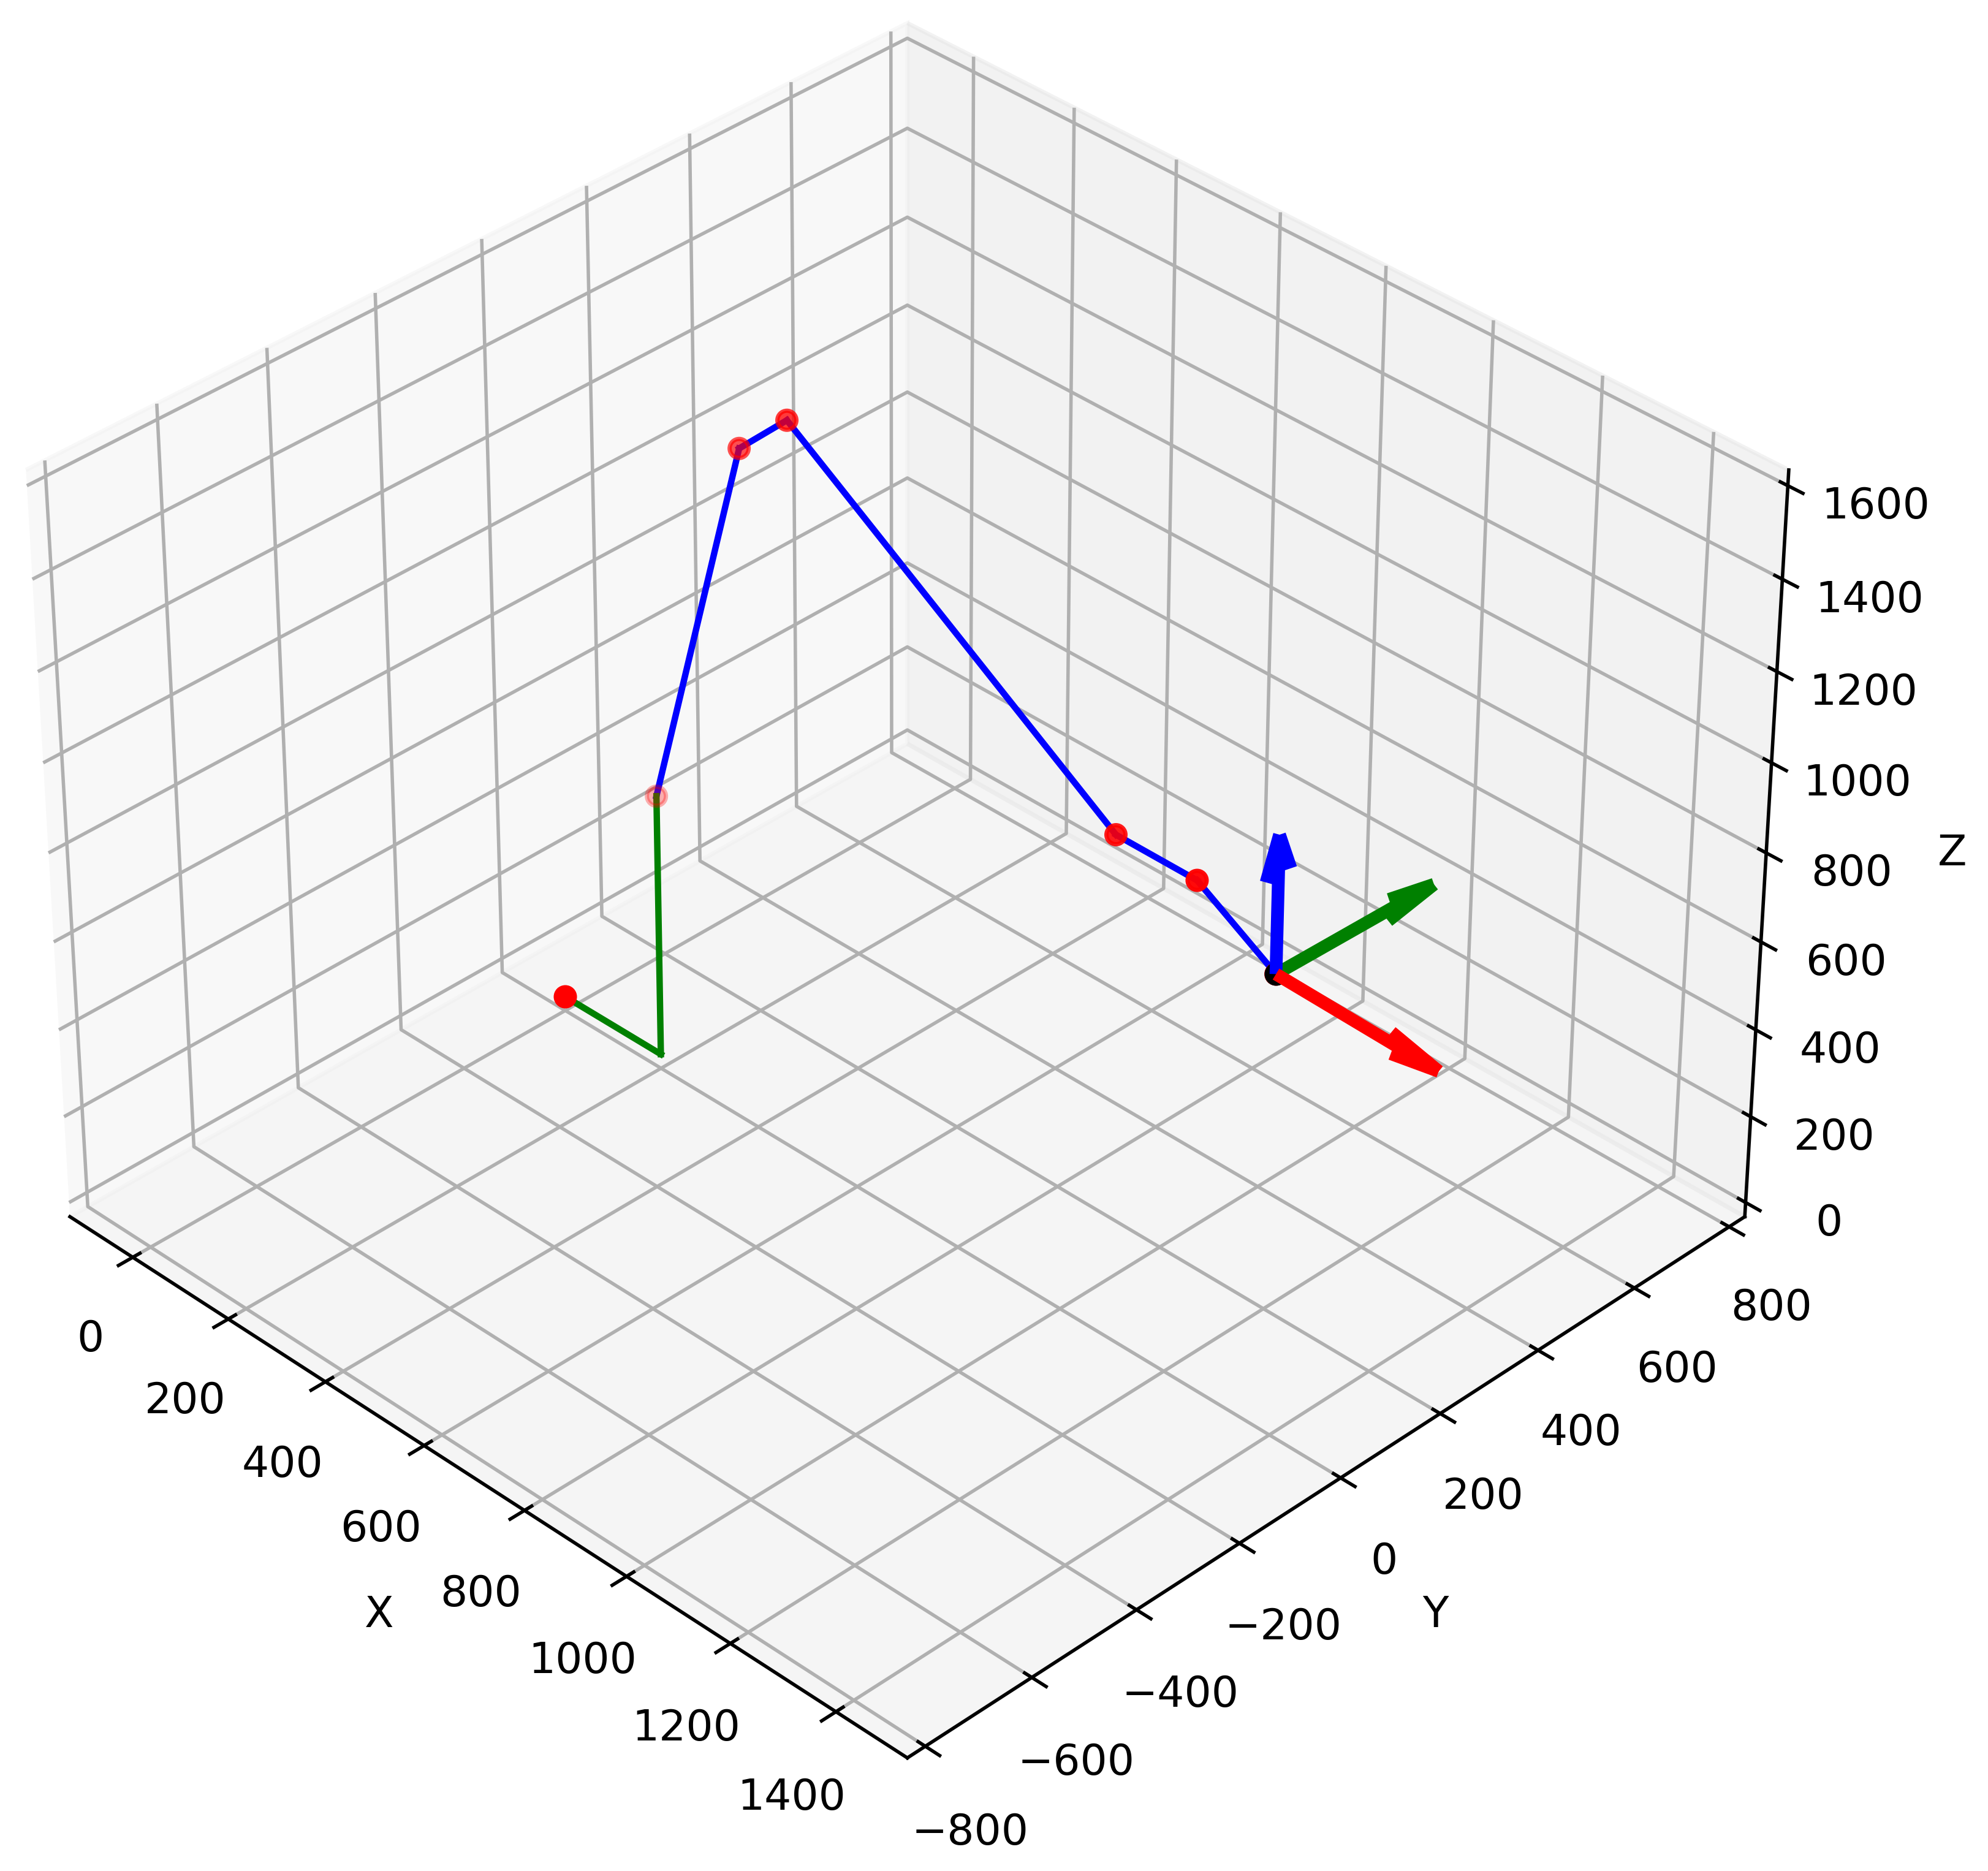
\includegraphics[width=0.9\textwidth]{figures/robotprog.png}}
	\caption{Visualization of the modeled robot}
	\label{robotprog}
\end{figure}


The arrows represent the coordinate axis of the TCP. For simplicity, the TCP is equal to the end point of the last joint. The X-axis is shown in red while the green and blue are the Y-axis and Z-axis respectively. The first link is shown in green and originates at the point~X=0~Y=0~Z=0.


The schematic of the modeled robot is shown in Figure \ref{schema}. In this configuration, all joints are in their initial position without any rotation.
\begin{figure}[H]
	\centerline{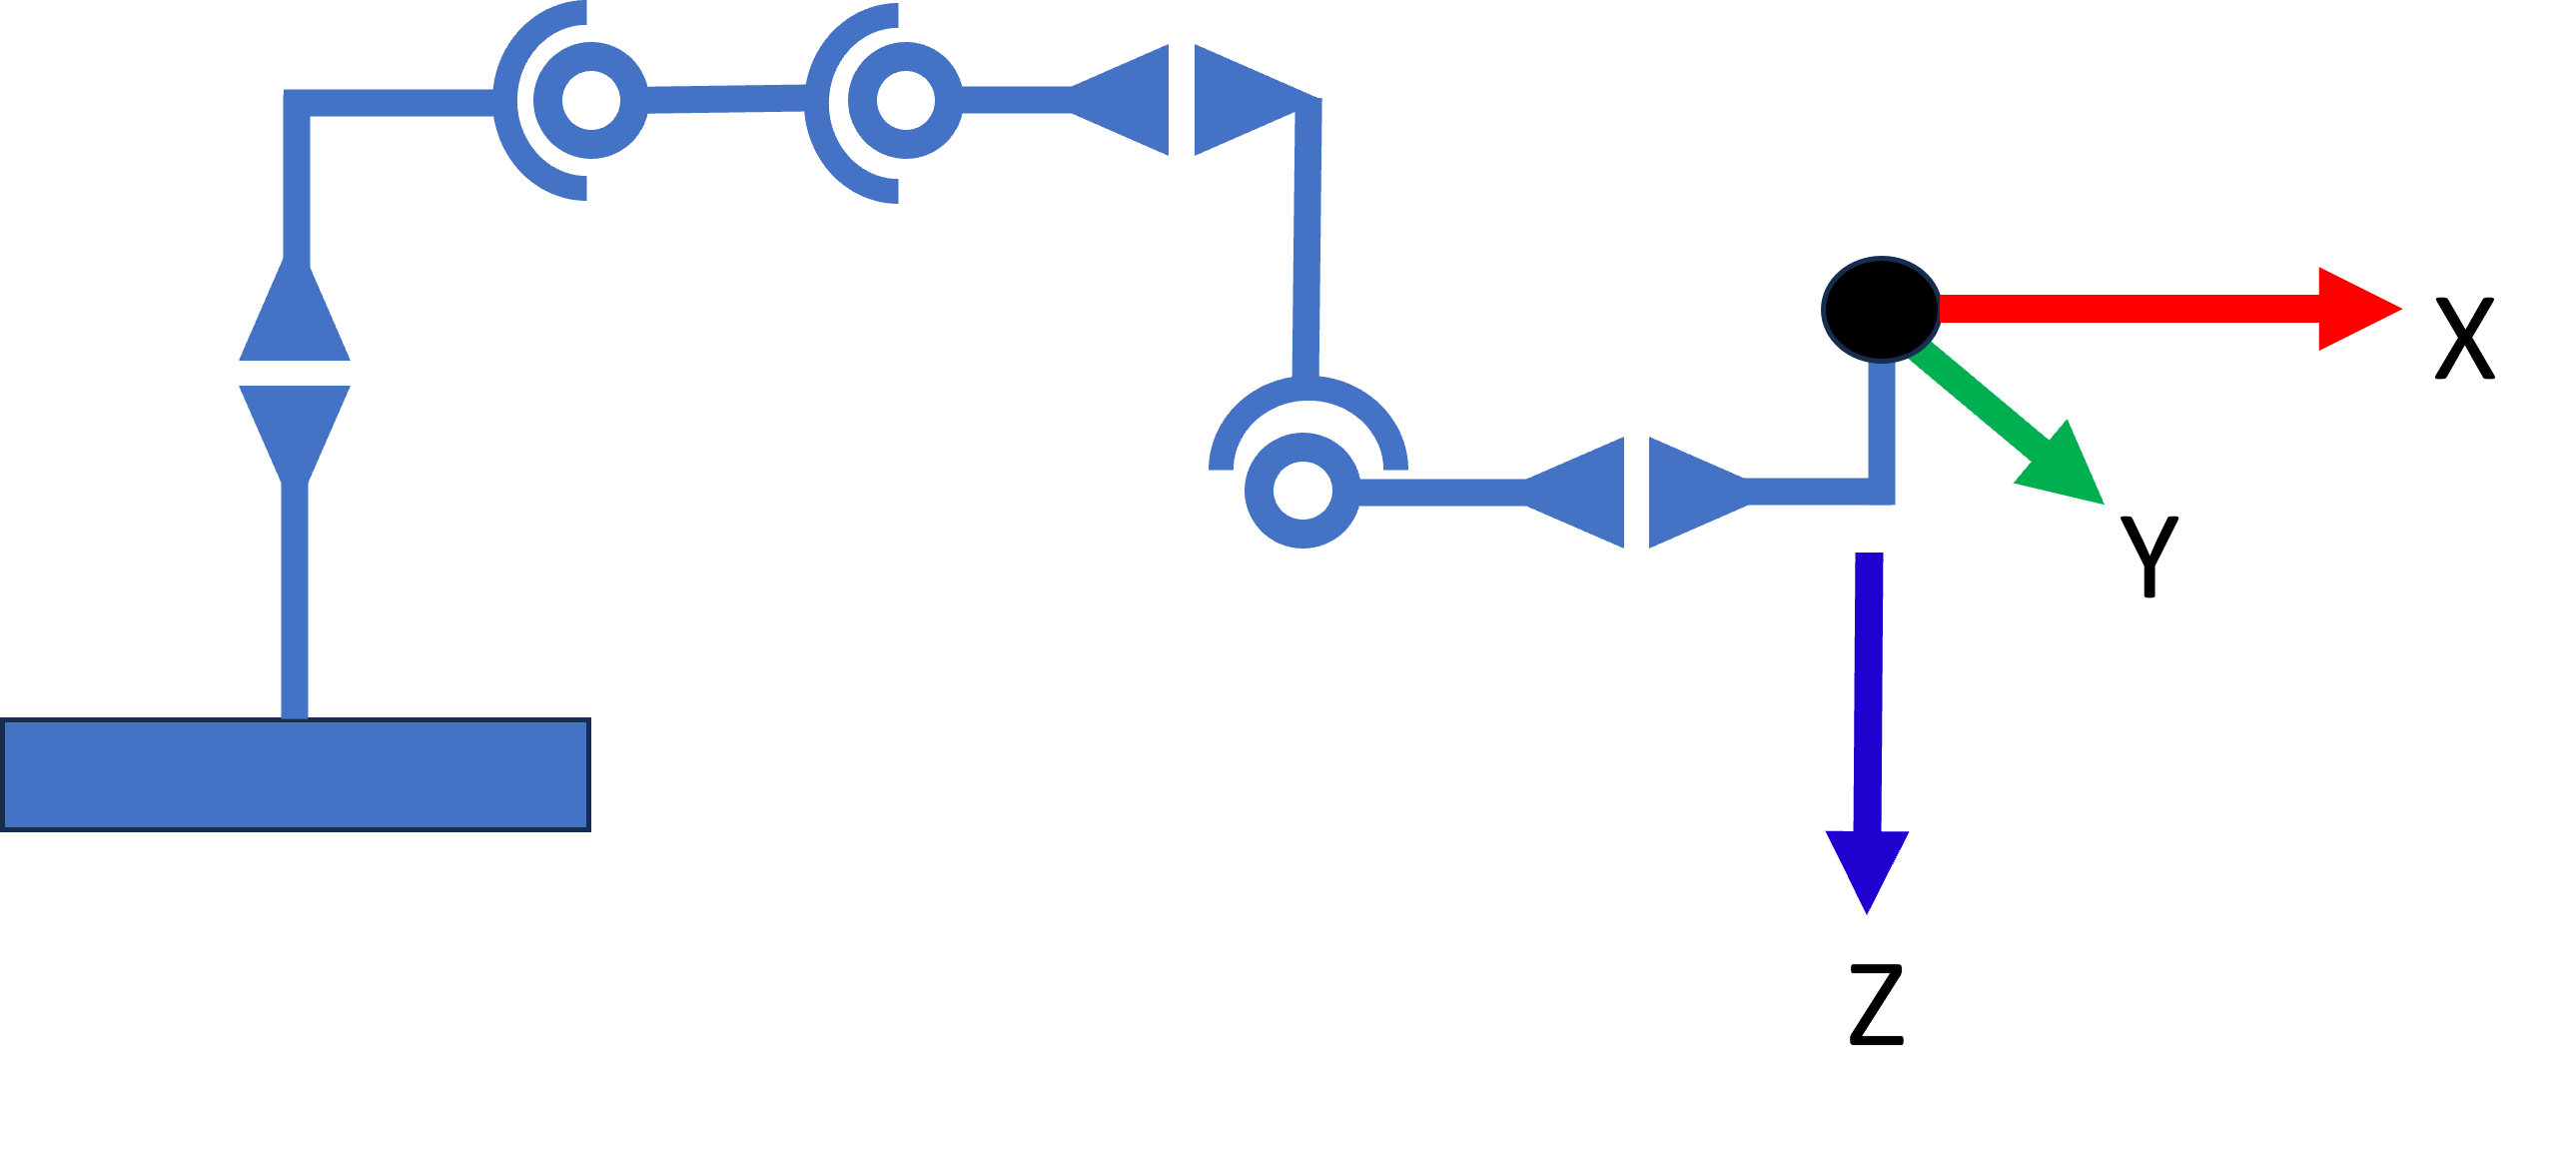
\includegraphics[width=0.7\textwidth]{figures/schema.png}}
	\caption{Schematics of the modeled robot}
	\label{schema}
\end{figure}

\subsection{Modeling a basic Toolpath}\label{MBT}
Before the process parameters can be analyzed, a toolpath needs to be defined for the TCP to follow. In this particular case, three possible options are presented. Each toolpath consists of 3000 coordinates. It is important to note that in these cases, the redundant DoF is the rotation around the C-Axis. This means that  this rotation will be adjusted to identify the most optimal value for the desired outcome.


The first toolpath, shown in Figure \ref{path1}, depicts a converging and diverging spiral. Figure \ref{path2} illustrates a converging loop, and Figure \ref{path3} displays a forward-moving sinusoidal curve. 

The corresponding equations are represented by Equation \ref{eq1}, Equation \ref{eq2}, and Equation \ref{eq3}. The variable \textit{iter} increments from 0 to 3000 and is used to calculate the X-Y-Z coordinates. The trigonometric functions are implemented using the \textit{Numpy} library.


\begin{equation}\label{eq1}
\begin{split}
x &= np.cos(np.deg2rad(iter)) * (500 - iter / 3)\\
y &= np.sin(np.deg2rad(iter)) * (500 - iter / 3)\\
z &= iter / 10
\end{split}
\end{equation}


\begin{equation}\label{eq2}
\begin{split}
x &= np.sin(np.deg2rad(iter)) * (400-iter / 5)\\
y &= np.sin(np.deg2rad(iter)) * np.cos(np.deg2rad(iter)) * (500-iter / 6)\\
z &= iter / 10
\end{split}
\end{equation}

\begin{equation}\label{eq3}
\begin{split}
x &= np.sin(np.deg2rad(iter)) * 200\\
y &= iter / 3 - (2500/3/2)\\
z &= np.sin(np.deg2rad(x))*100
\end{split}
\end{equation}


\begin{figure}[H]% [H] is so declass\'e!
	\centering
	\begin{minipage}{0.5\textwidth}
		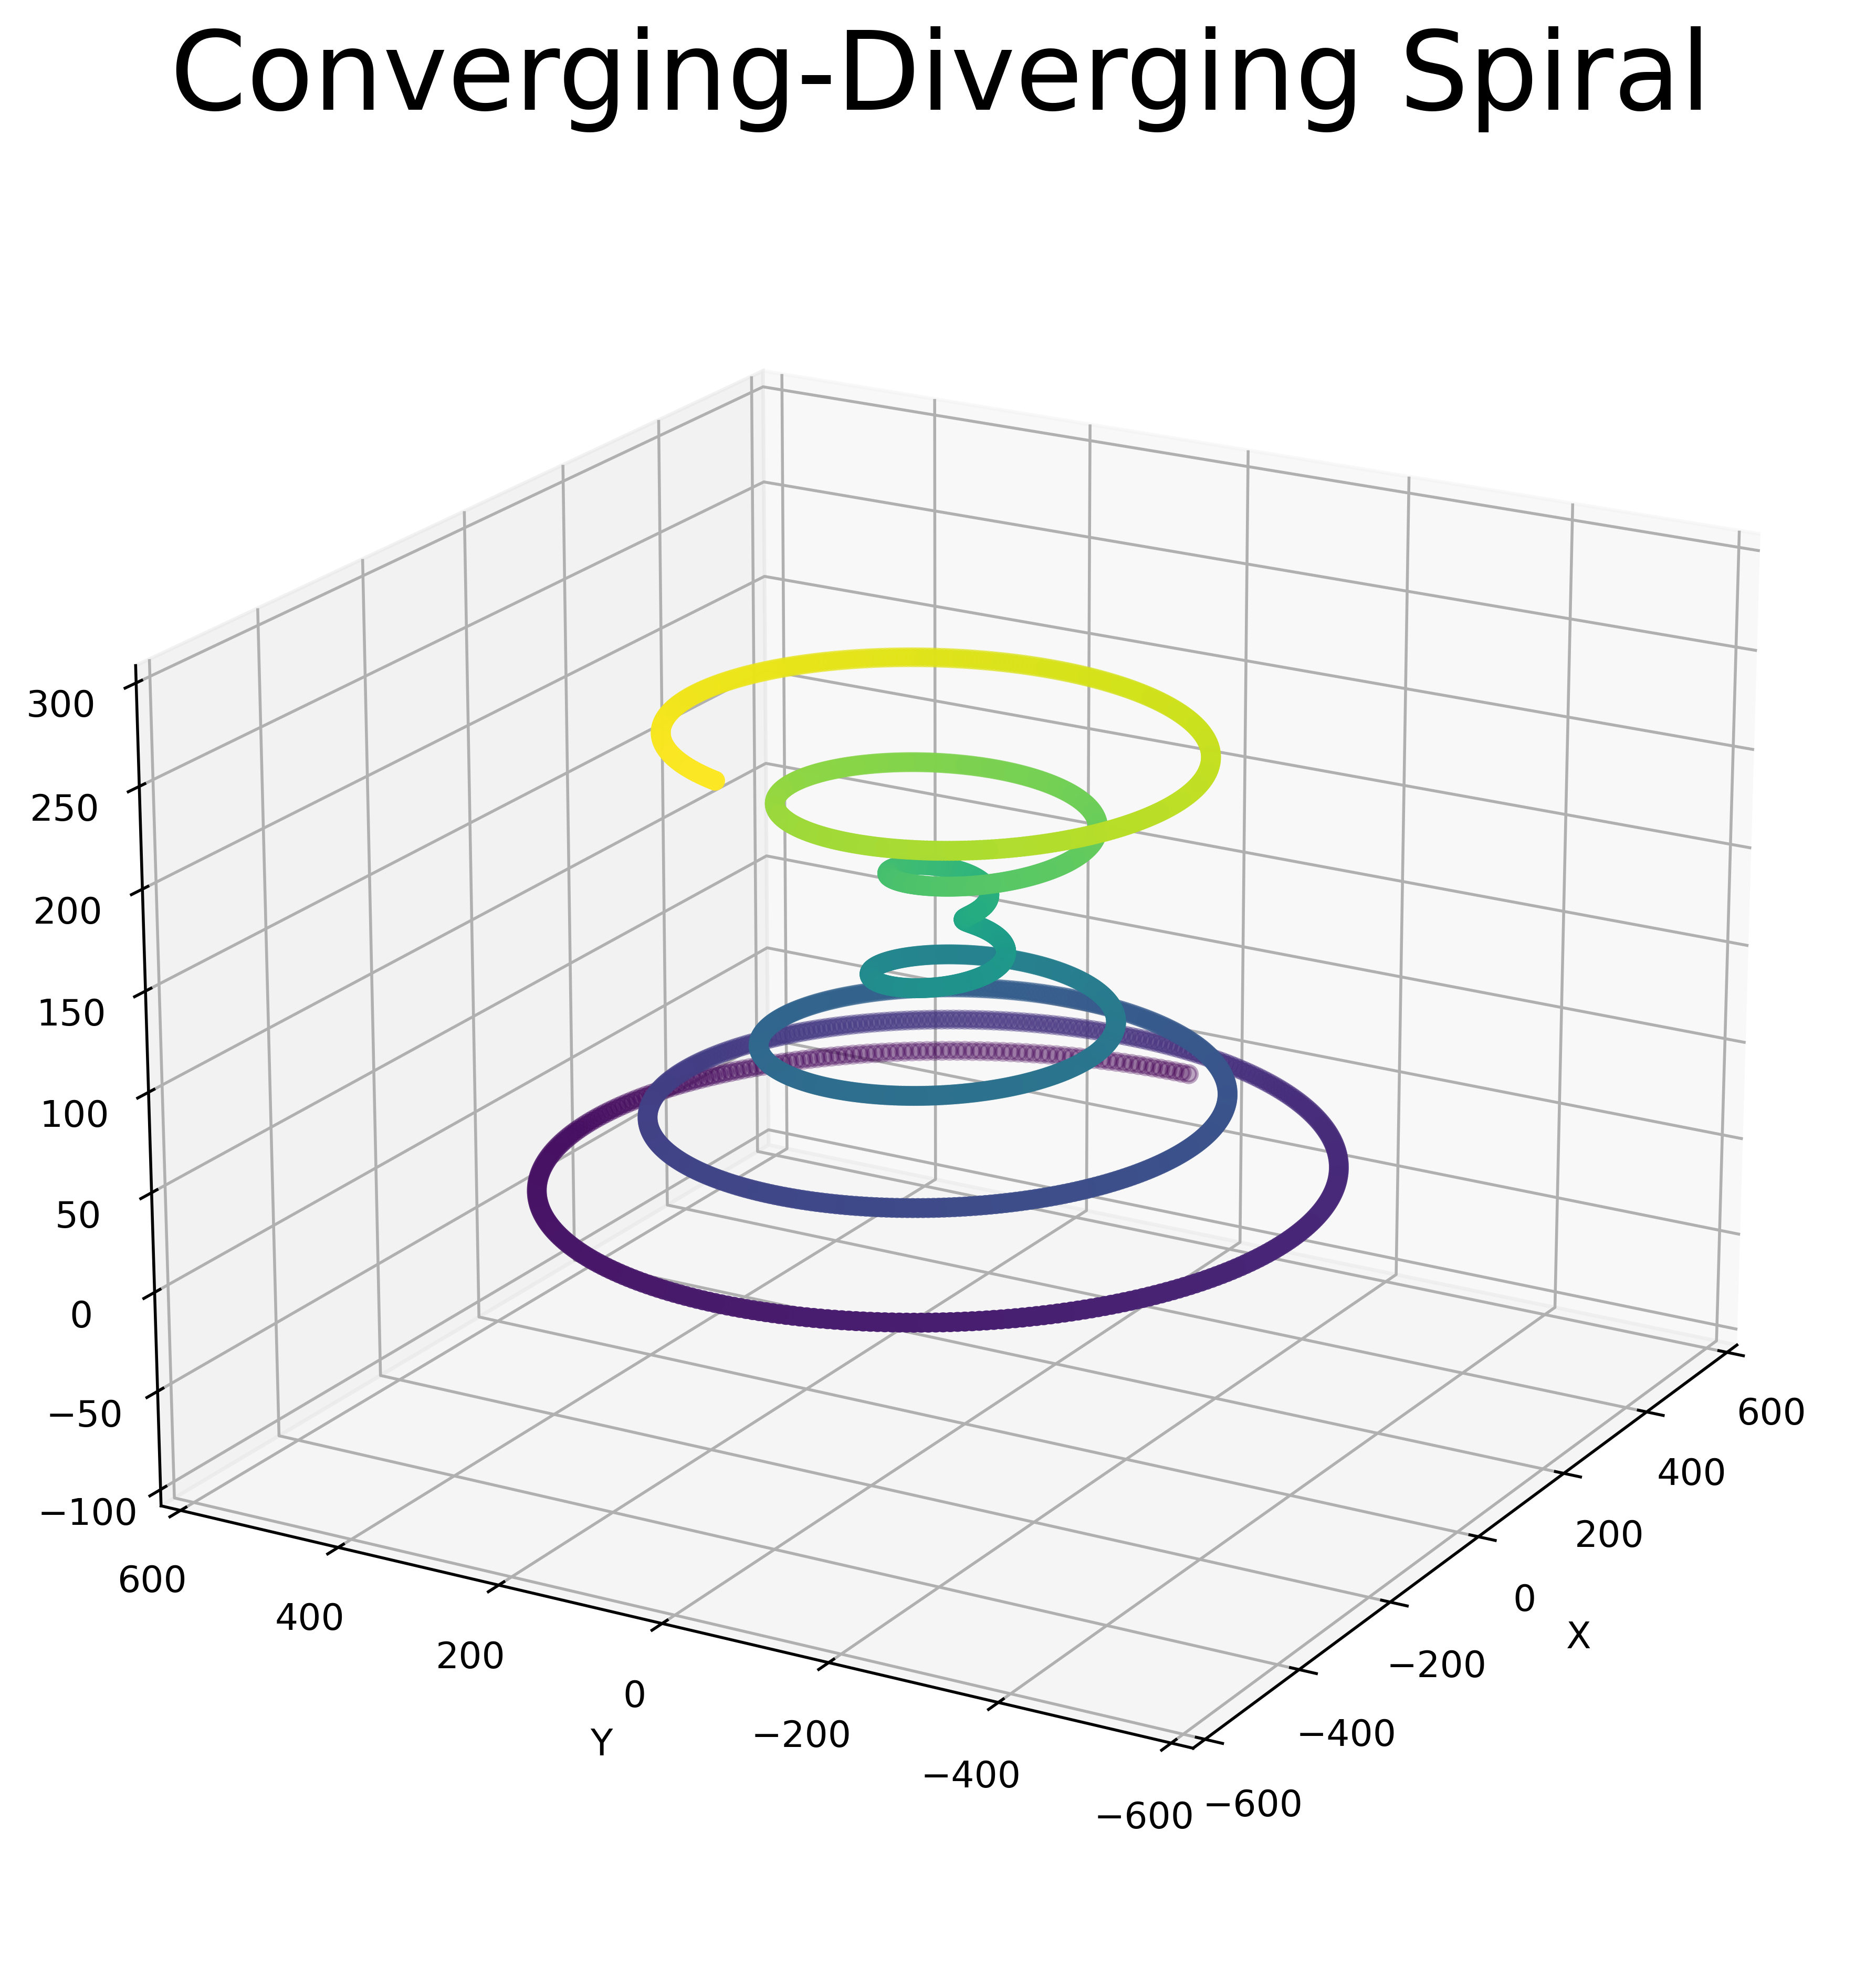
\includegraphics[width=\textwidth]{figures/path1.png}
		\caption{Toolpath 1: Converging-Diverging Spiral}
		\label{path1}
	\end{minipage}\hfill
	\begin{minipage}{0.5\textwidth}
		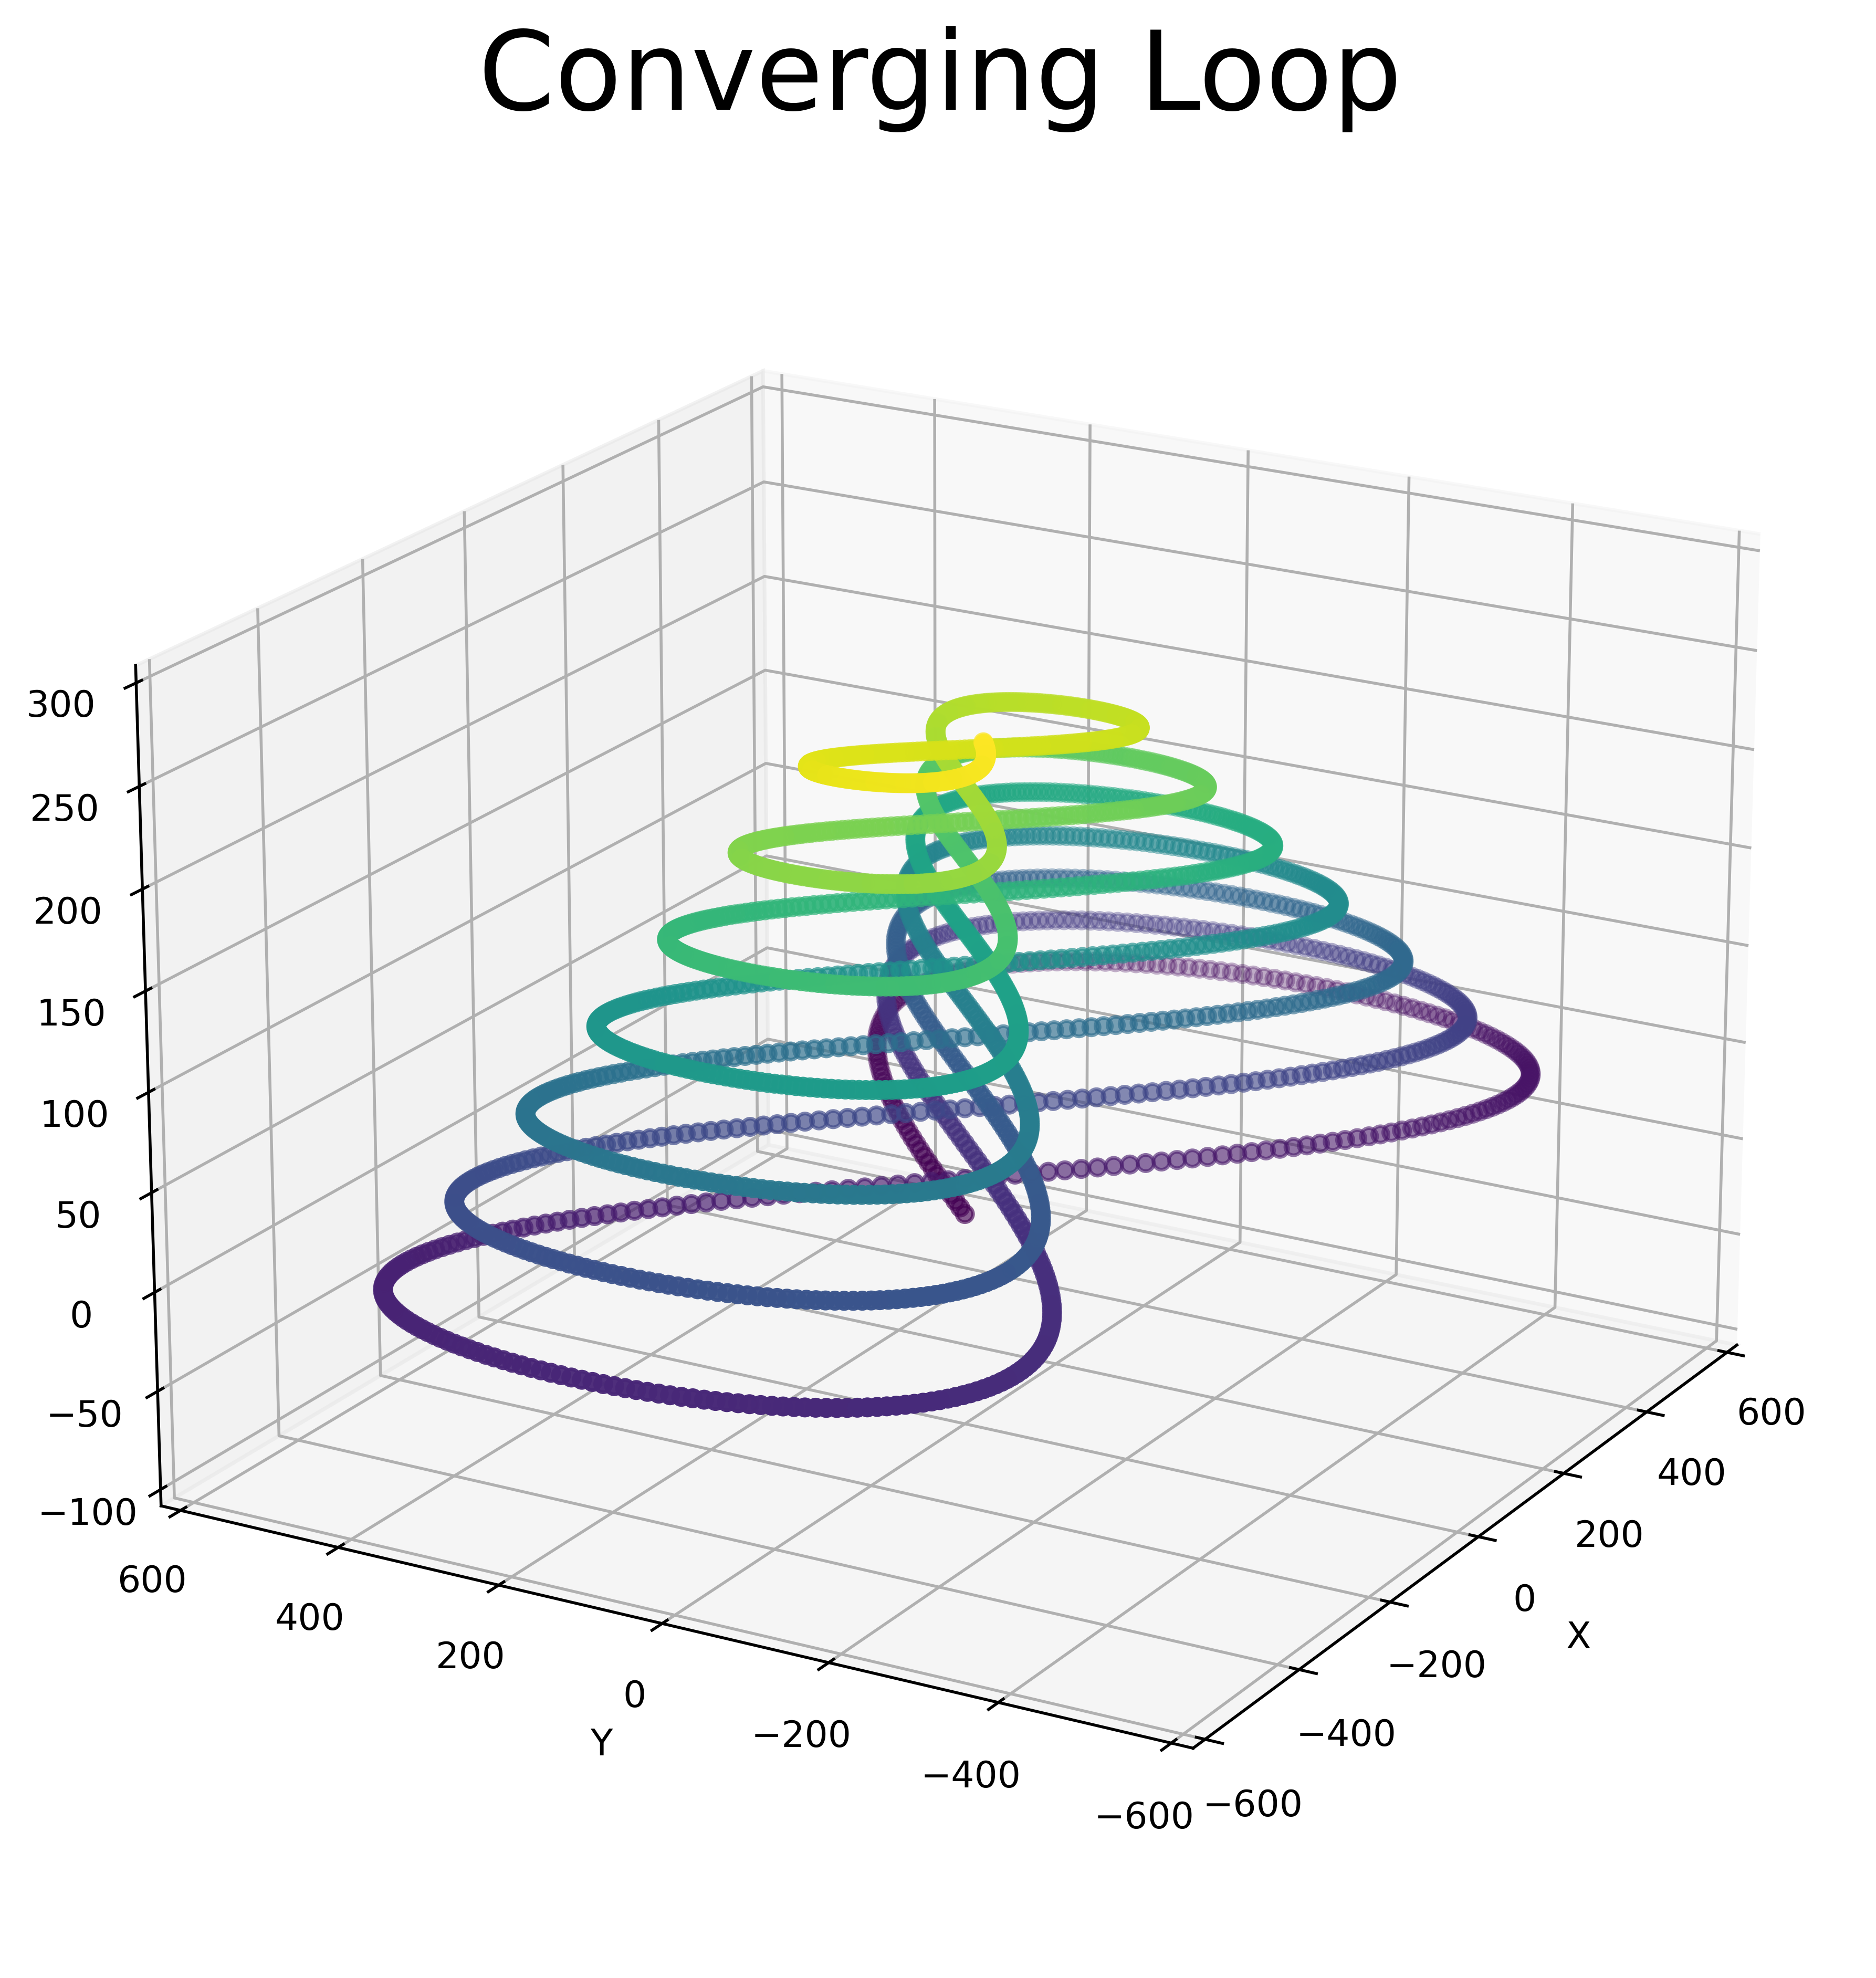
\includegraphics[width=\textwidth]{figures/path2.png}
		\caption{Toolpath 2: Converging Loop}
		\label{path2}
	\end{minipage}\par
	\vskip\floatsep% normal separation between figures
	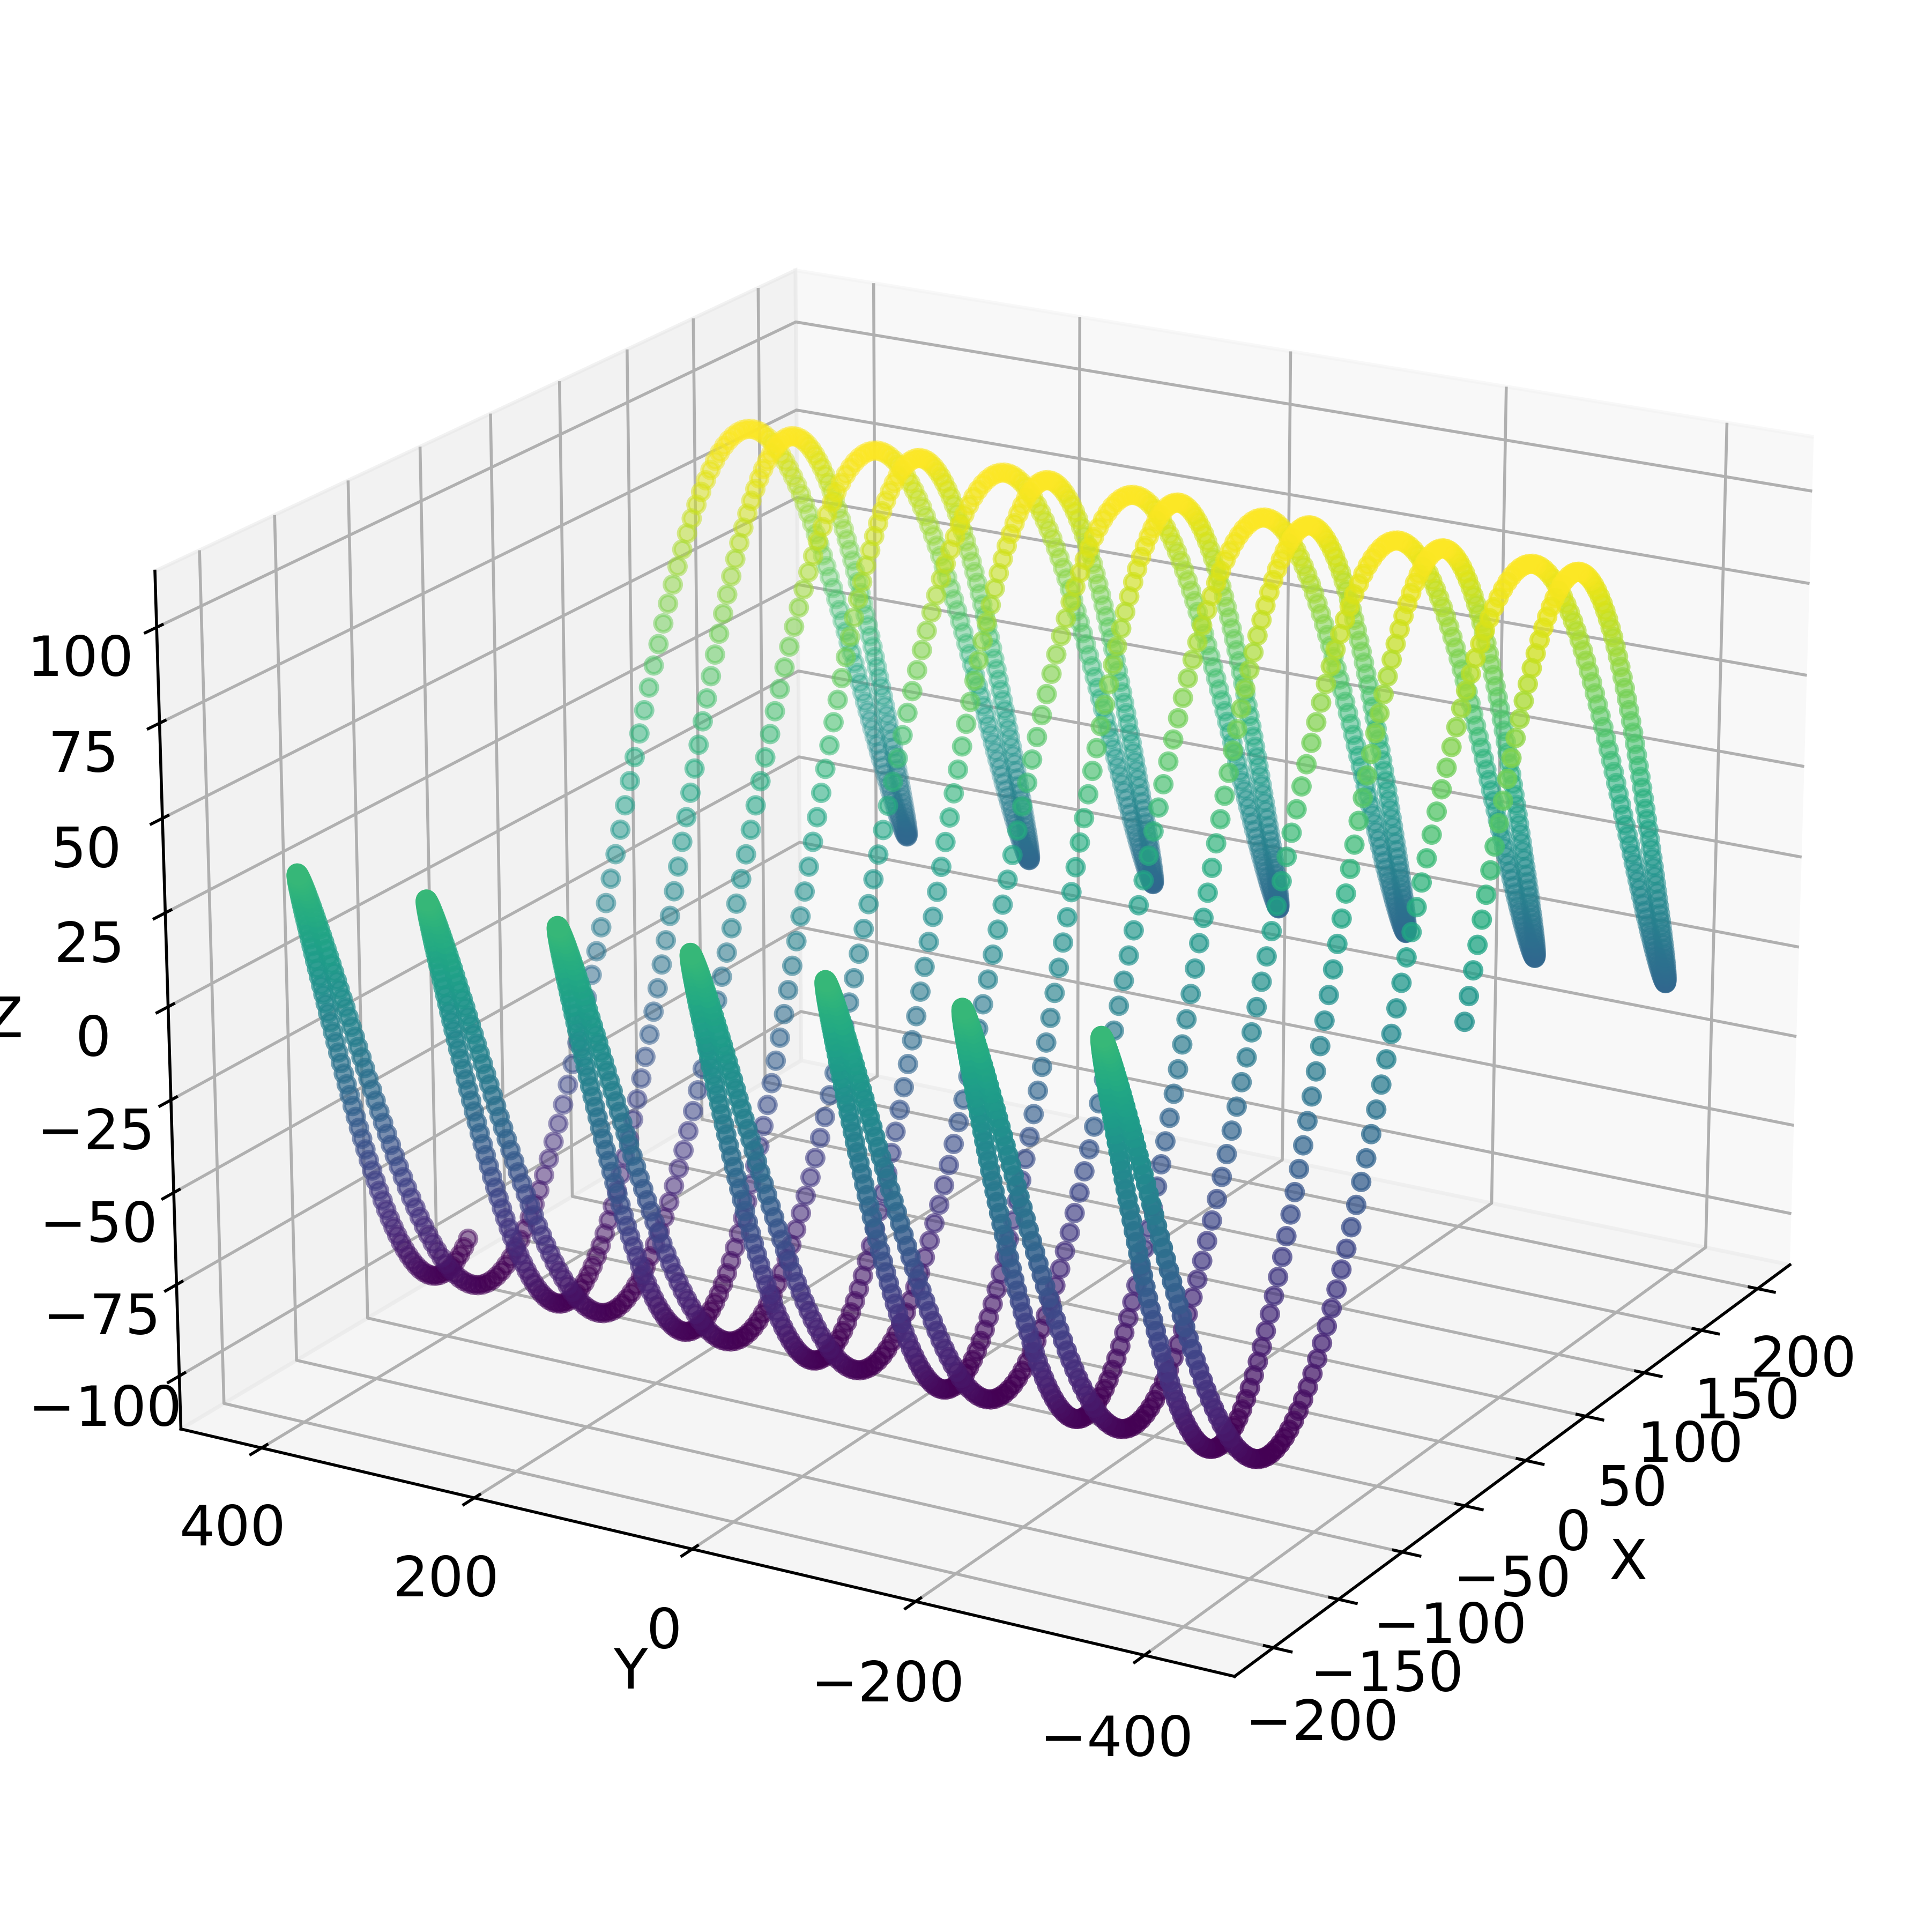
\includegraphics[width=0.5\textwidth]{figures/path3.png}

	\caption{Toolpath 3: Pendulum Oscillation}
	\label{path3}
\end{figure}

\newpage
Figure \ref{TP1robot} depicts the robot and Toolpath 1 (described by Equation \ref{eq1}) at the final position of the toolpath. The toolpath's origin is shifted by X=1000 and Z=600 relative to the robot's coordinate system. There is no rotation around axes X, Y, and Z. Thus A B and C is zero.

\begin{figure}[H]
	\centerline{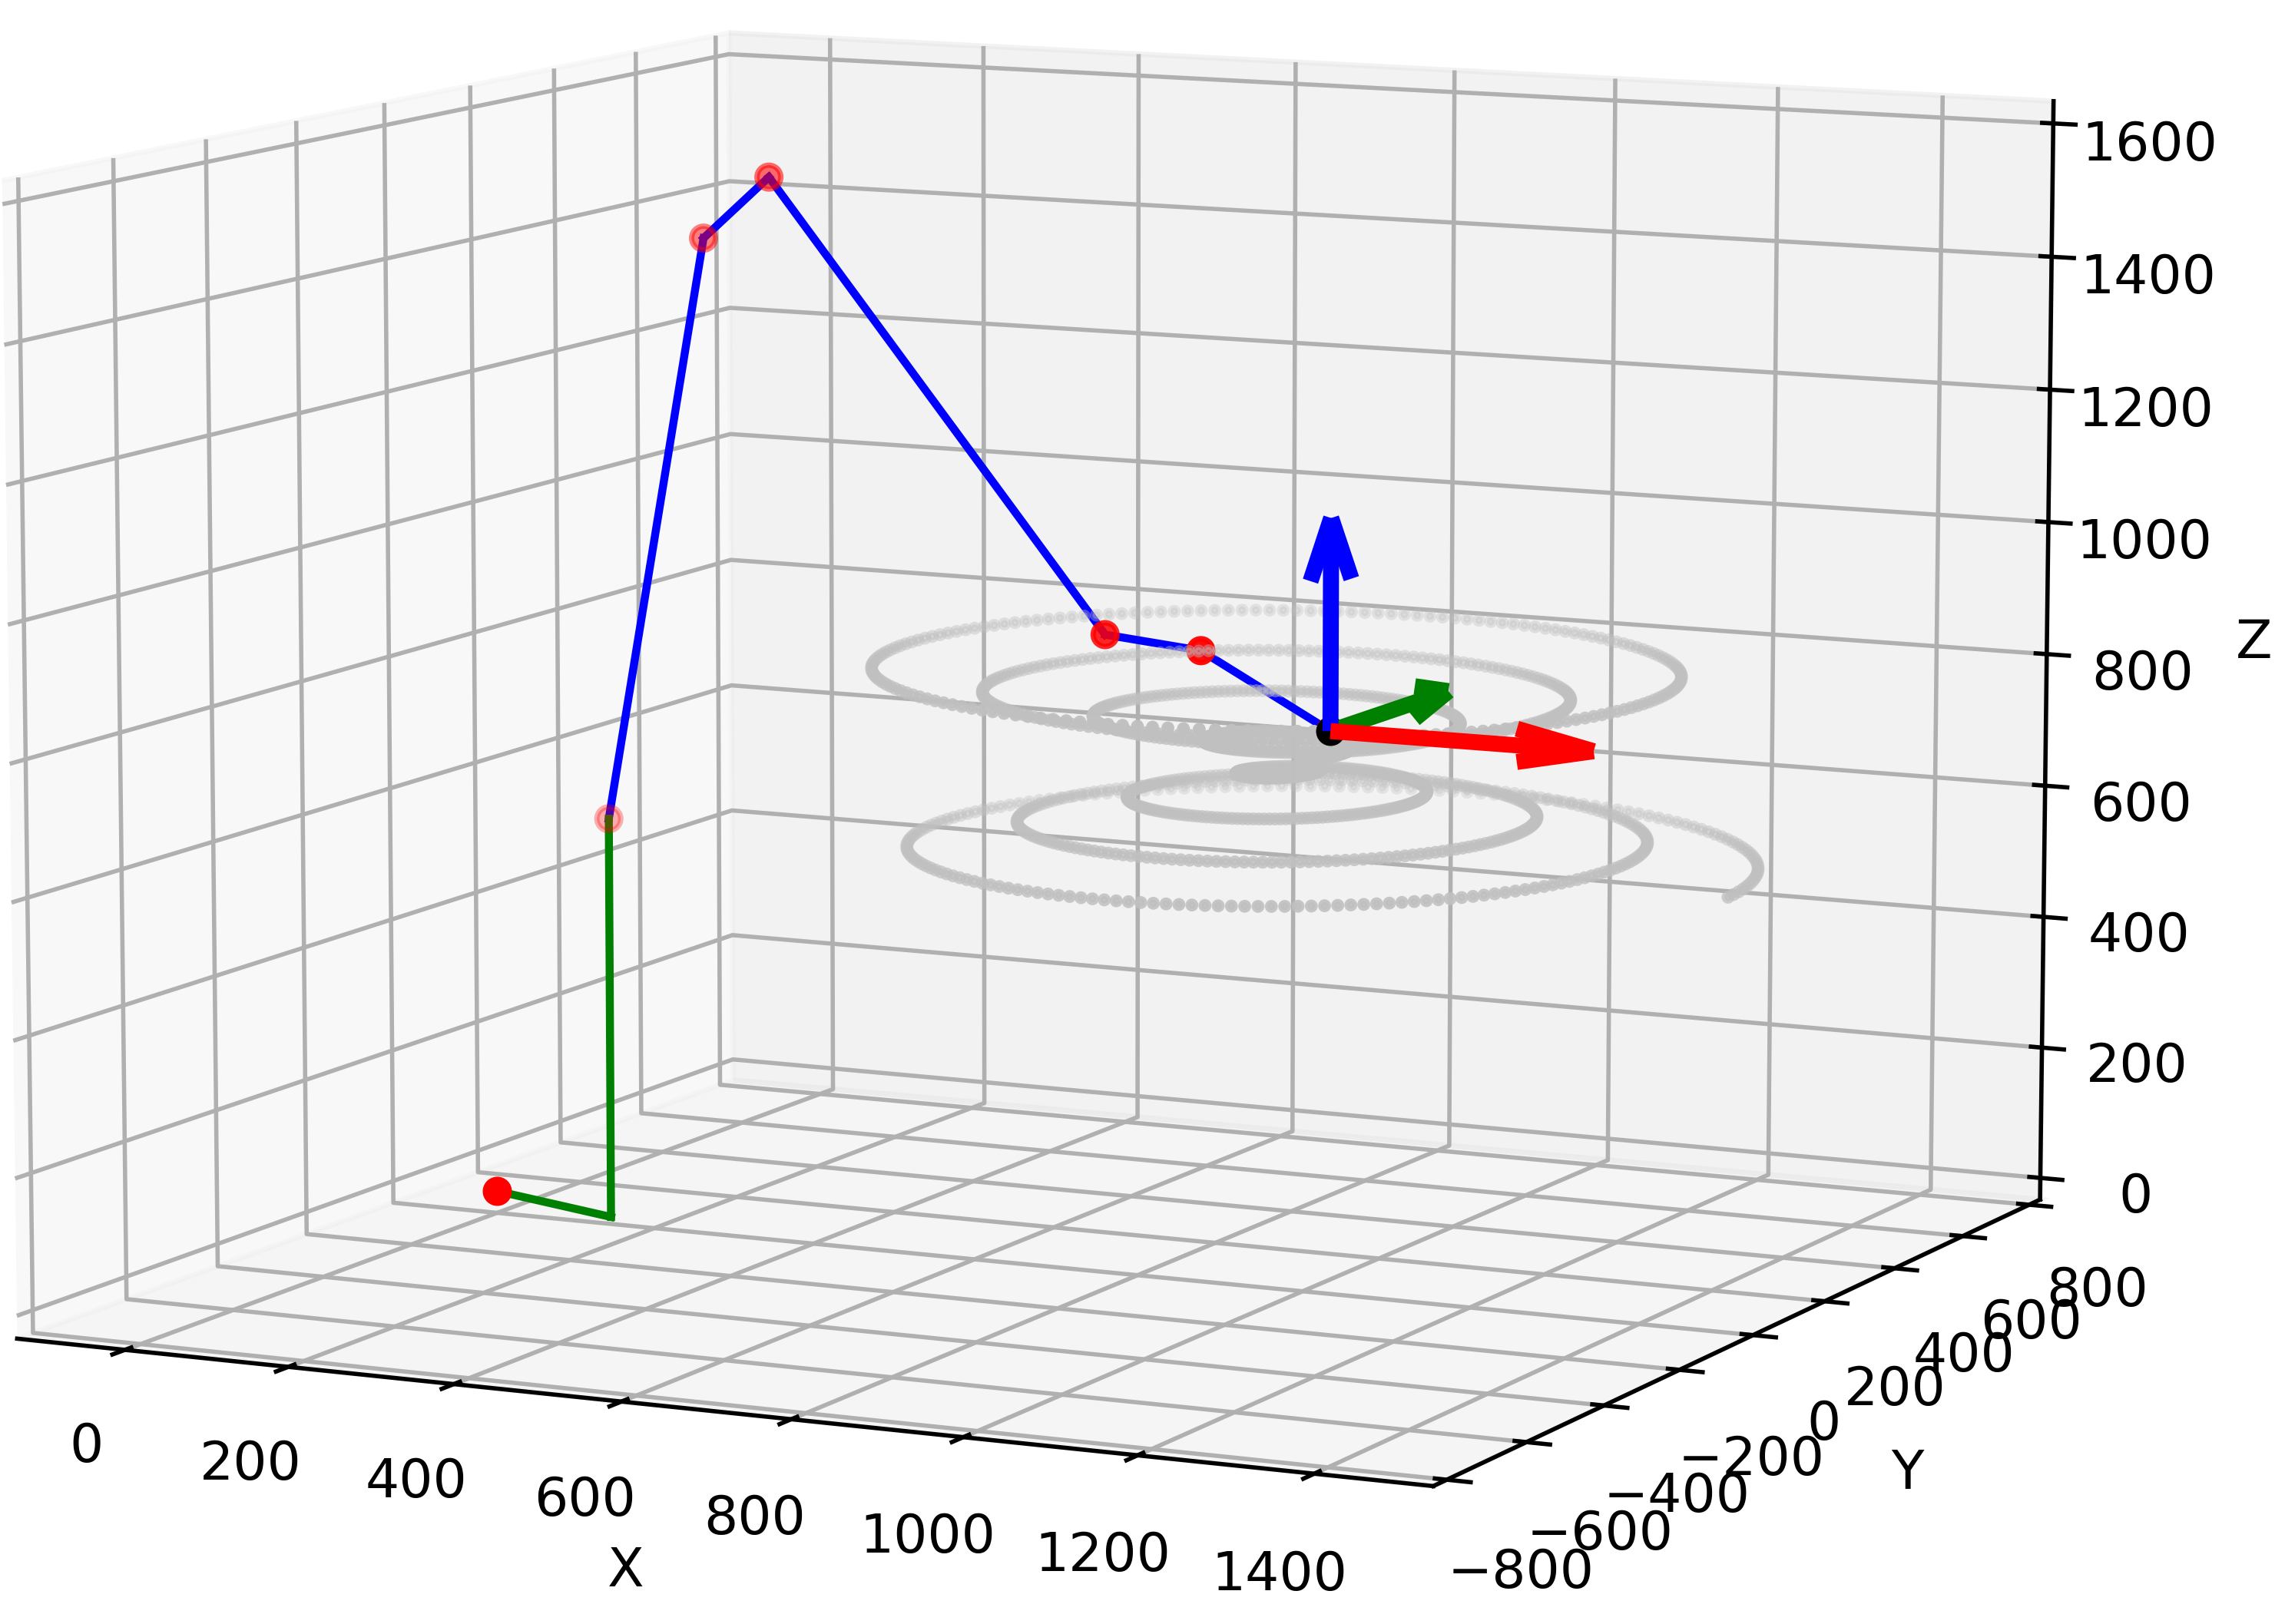
\includegraphics[width=0.9\textwidth]{figures/robotANDpath1.png}}
	\caption{Toolpath 1 with robot model}
	\label{TP1robot}
\end{figure}




\subsection{Extracting process parameters}
With the assistance of an inverse kinematics algorithm from the Python library \textit{visual\_kinematics}, the joint angles can be computed. The outcome is a time series containing the corresponding joint positions. Currently, all coordinates must be traversed in equidistant timesteps. With this information, it becomes feasible to calculate the velocity and other related parameters. After transforming all the data from the time series into scalar values and calculating the local score, the global score can be determined.
\newpage
\section{Testing and Validation}%

\subsection{Toolpath Evaluation with one Redundant DoF}
As mentioned in Chapter \ref{MBT}, the toolpath is considered constant in regards to the coordinates X-Y-Z. The fixed boundary conditions for the robot are that the rotations around the X and Y axes are 0. The user needs to set the degree of freedom for the rotation around the Z axis, which is the free degree of freedom. Figure \ref{TP1ABC0} illustrates the variation of each joint over time for toolpath 1. In this specific case, the rotations A, B, and C are set to 0. The whole toolpath is traversed in 300 seconds. 

\begin{figure}[H]
	\centerline{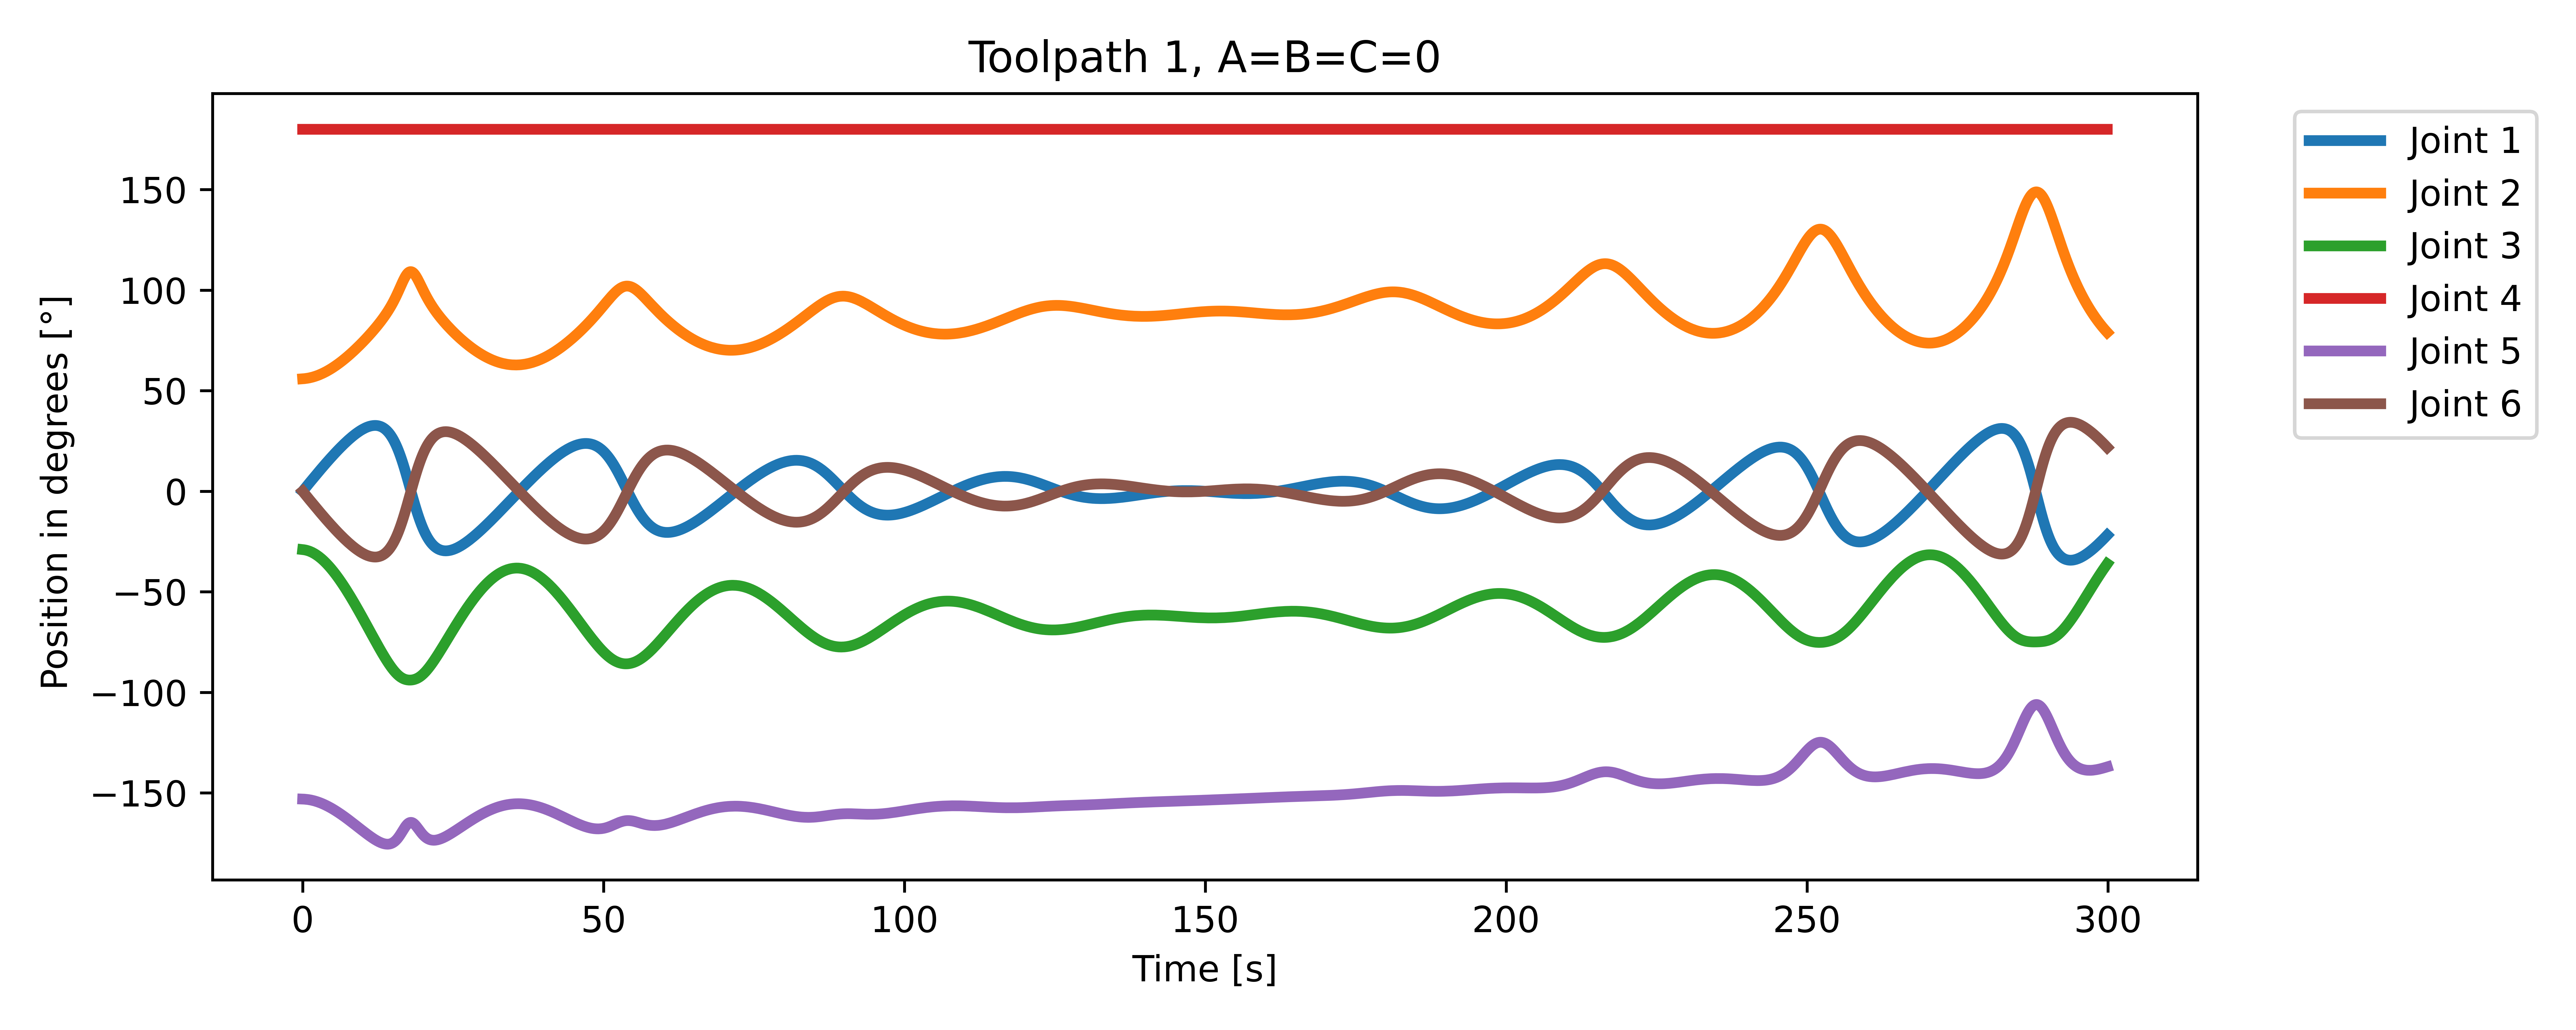
\includegraphics[width=1\textwidth]{figures/TP1ABC0.png}}
	\caption{xxx}
	\label{TP1ABC0}
\end{figure}
In this specific case, joints 1 and 6 oscillate out of phase relative to each other around a zero degrees. Joint 3 remains constantly at 180 degrees. Joint 2 and 5 also oscillate and slightly increase.


The next step is to establish the weights for each individual process parameter. Initially, a basic case is discussed. The selected process parameters can be found in table \ref{PPbasic}. The total number of direction changes in all joints is counted, and the total distance traveled is calculated. Both of these process parameters are given an importance rating of 0.4. Additionally, the acceleration of joint 1 is analyzed. To obtain a scalar value for the acceleration, the individual values are squared and then summed. Velocity, acceleration, and jerk are disregarded for all other joints.

\begin{table}[H]
	\centering
	\begin{tabular}{||l|l||}
		Process parameters& Importance Factor \\
		\hline
		\hline
		\hline
		Direction changes in joints 1-6	&		0.4 \\
		Total travel in joints 1-6	&  	0.4 \\
		acceleration in joint 1	& 		0.2\\
		
		\hline
		\hline
	\end{tabular}
	
	\caption{xxx}
	\label{PPbasic}
\end{table}


As only a single DoF is being analyzed, it is possible to display the individual local scores and global score as a one-dimensional graph. Initially, toolpath 1 is analyzed, with the unconstrained DoF incremented by 0.01 radians. The starting value for the rotation around the Z axis is set to 0.8 radians. A total of 175 time series of joint positions are generated, and the process parameters are extracted and scaled in relation to each other. It is important to note that the selected process parameters are premultiplied by -1 because each process parameter should be minimized.

Following this, the local scores of each process parameter can be plotted as a one-dimensional graph, as shown in figure \ref{LS1}. It can be seen that the local scores of the selected process parameters have a significant dip in the range from -0.3 rad and 0.3 rad.

\begin{figure}[H]
	\centerline{
\includegraphics[width=1\textwidth]{figures/LocalScores_1.png}}
	\caption{xxx}
	\label{LS1}
\end{figure}


The arrays of the local scores are multiplied by the weights selected in table \ref{PPbasic} and then summed up. The resulting array shows the global score achieved by setting the rotation around the Z axis relative to all other analyzed values. The green dot indicates the maximum achievable score and its corresponding rotation in radians.
Even though the section ranging from -0.3 rad to 0.3 rad has significantly more low global scores, the best possible score with 98.1 is achieved at 0.1 radians.

\begin{figure}[H]
	\centerline{\includegraphics[width=1\textwidth]{figures/best_c_1.png}}
	\caption{xxx}
	\label{GS1}
\end{figure}


Insert tollpath 2  here

\subsection{Toolpath Evaluation with two Redundant DoF}
\begin{figure}[H]% [H] is so declass\'e!
	\centering
	\begin{minipage}{0.5\textwidth}
		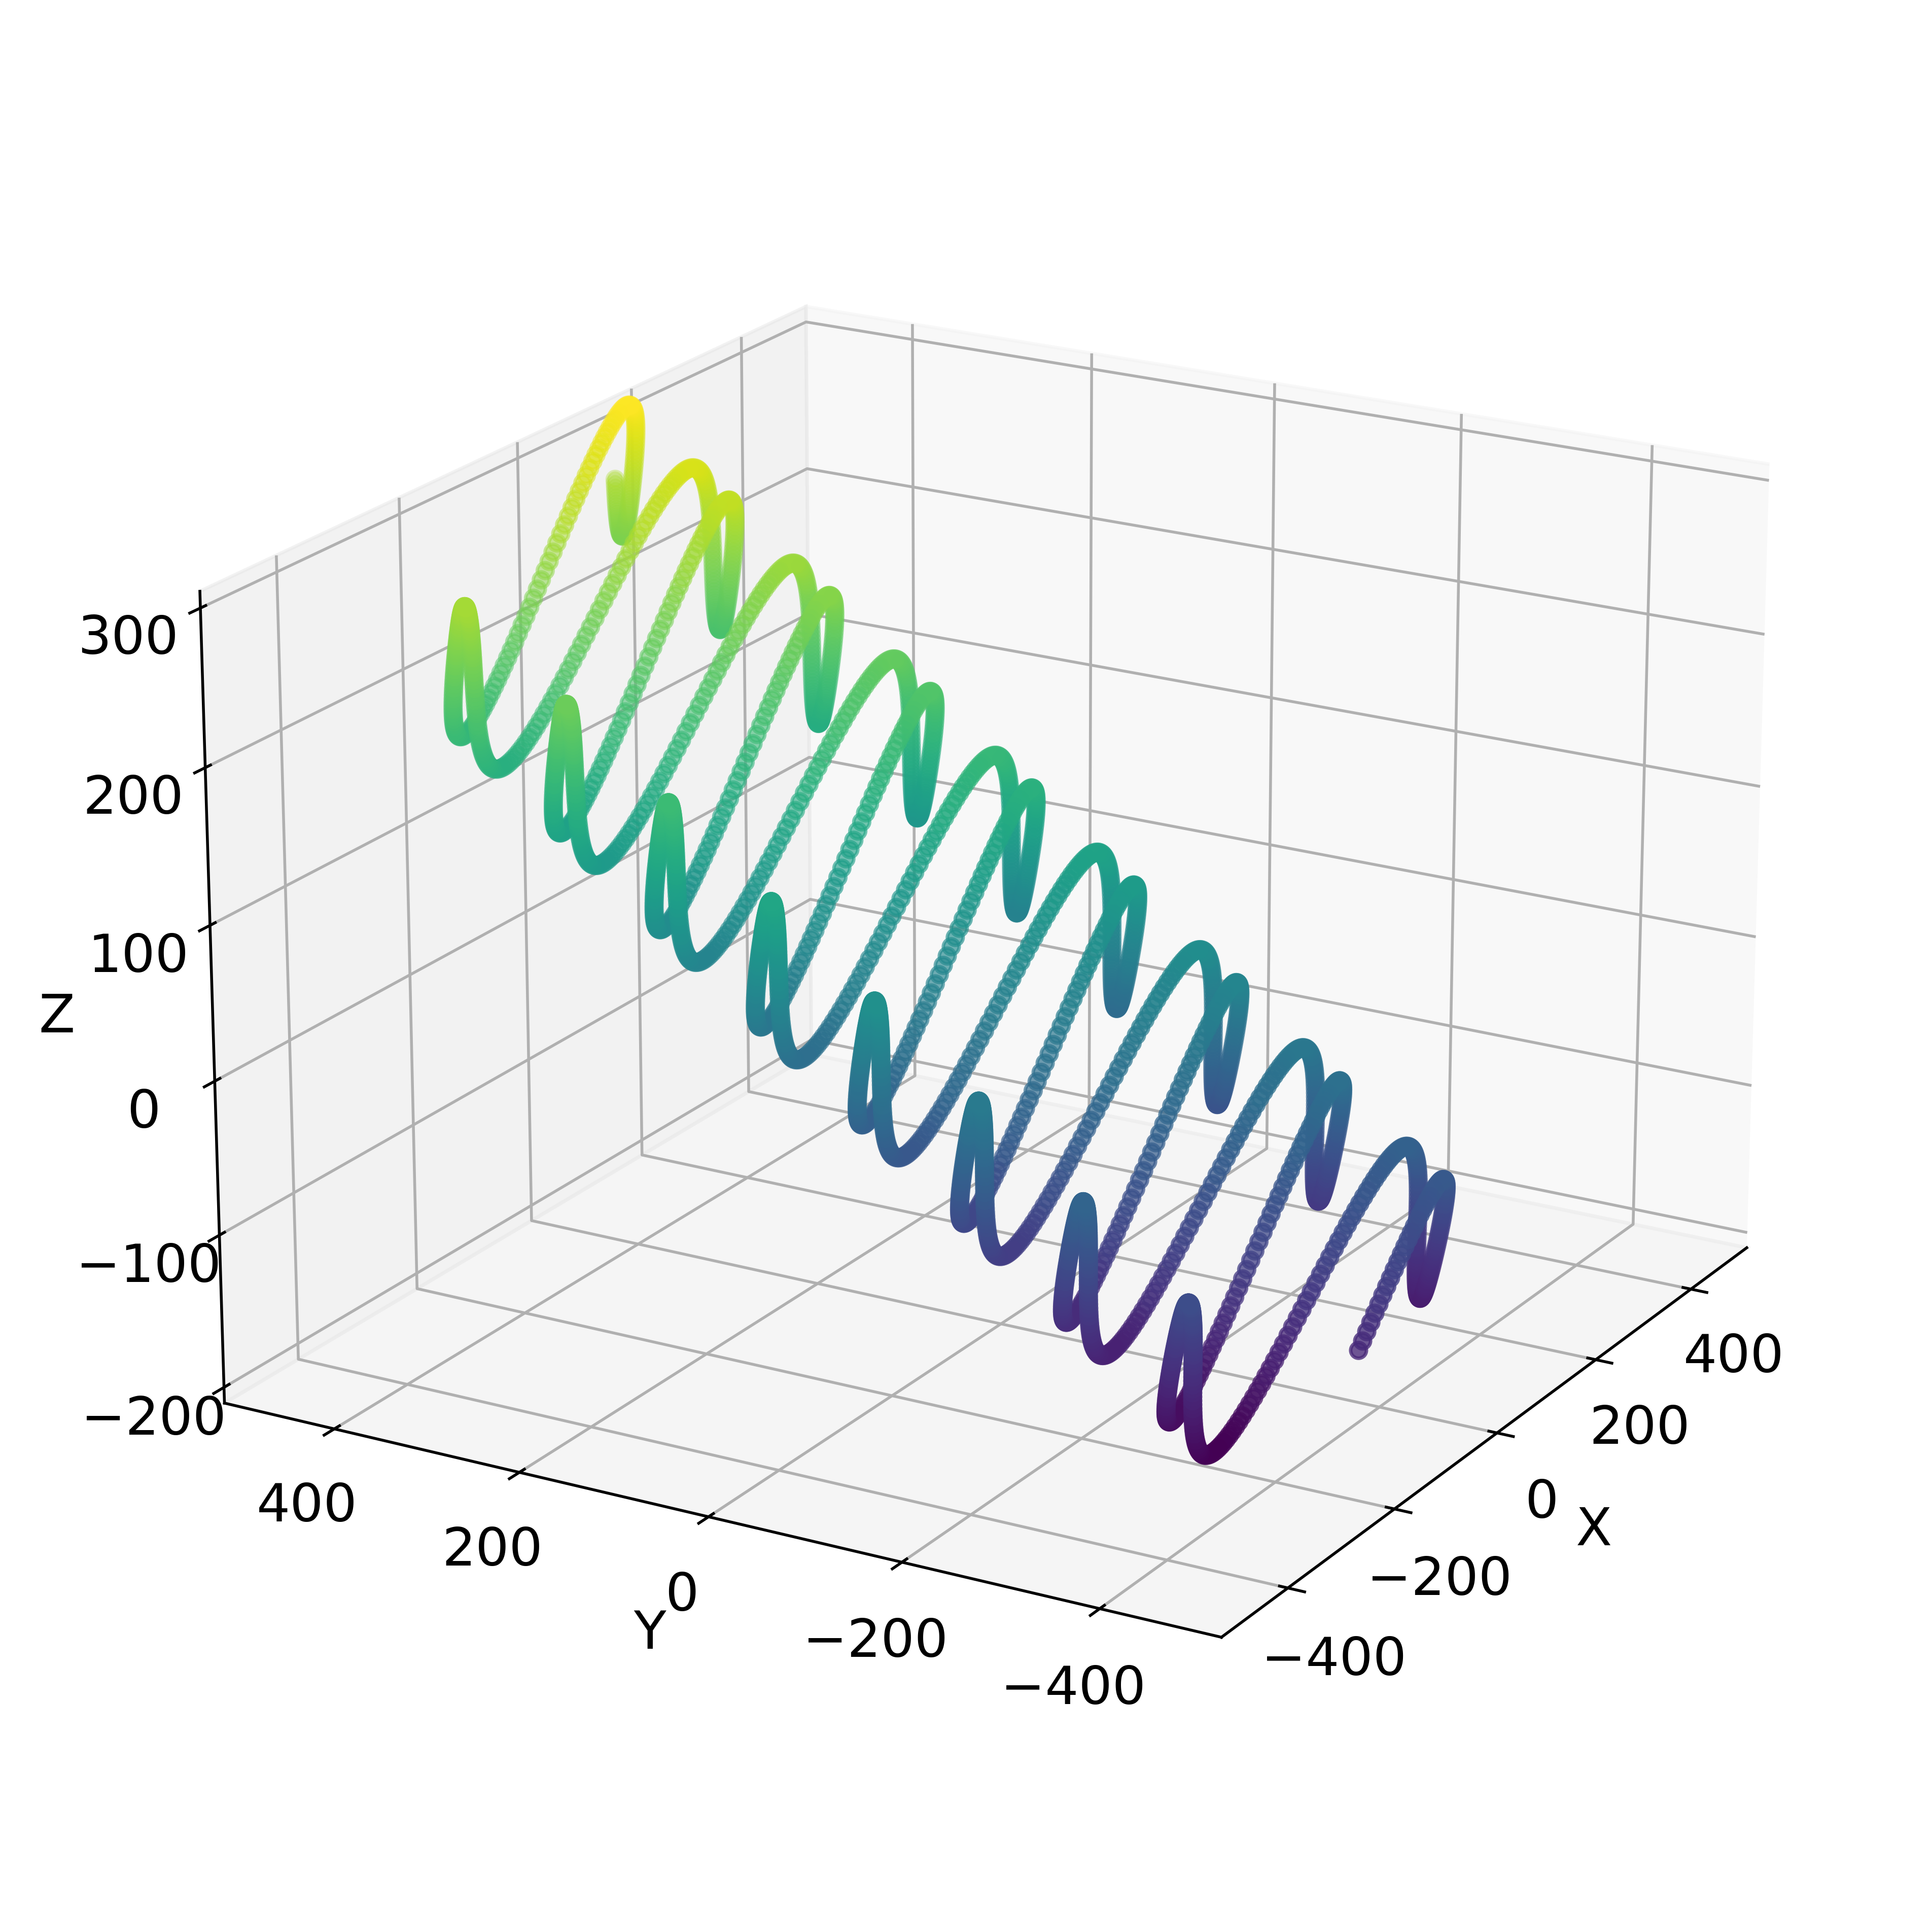
\includegraphics[width=\textwidth]{figures/path3_kipp_25.png}
		\caption{sdfgsdf}
		\label{asdsdfg}
	\end{minipage}\hfill
	\begin{minipage}{0.5\textwidth}
		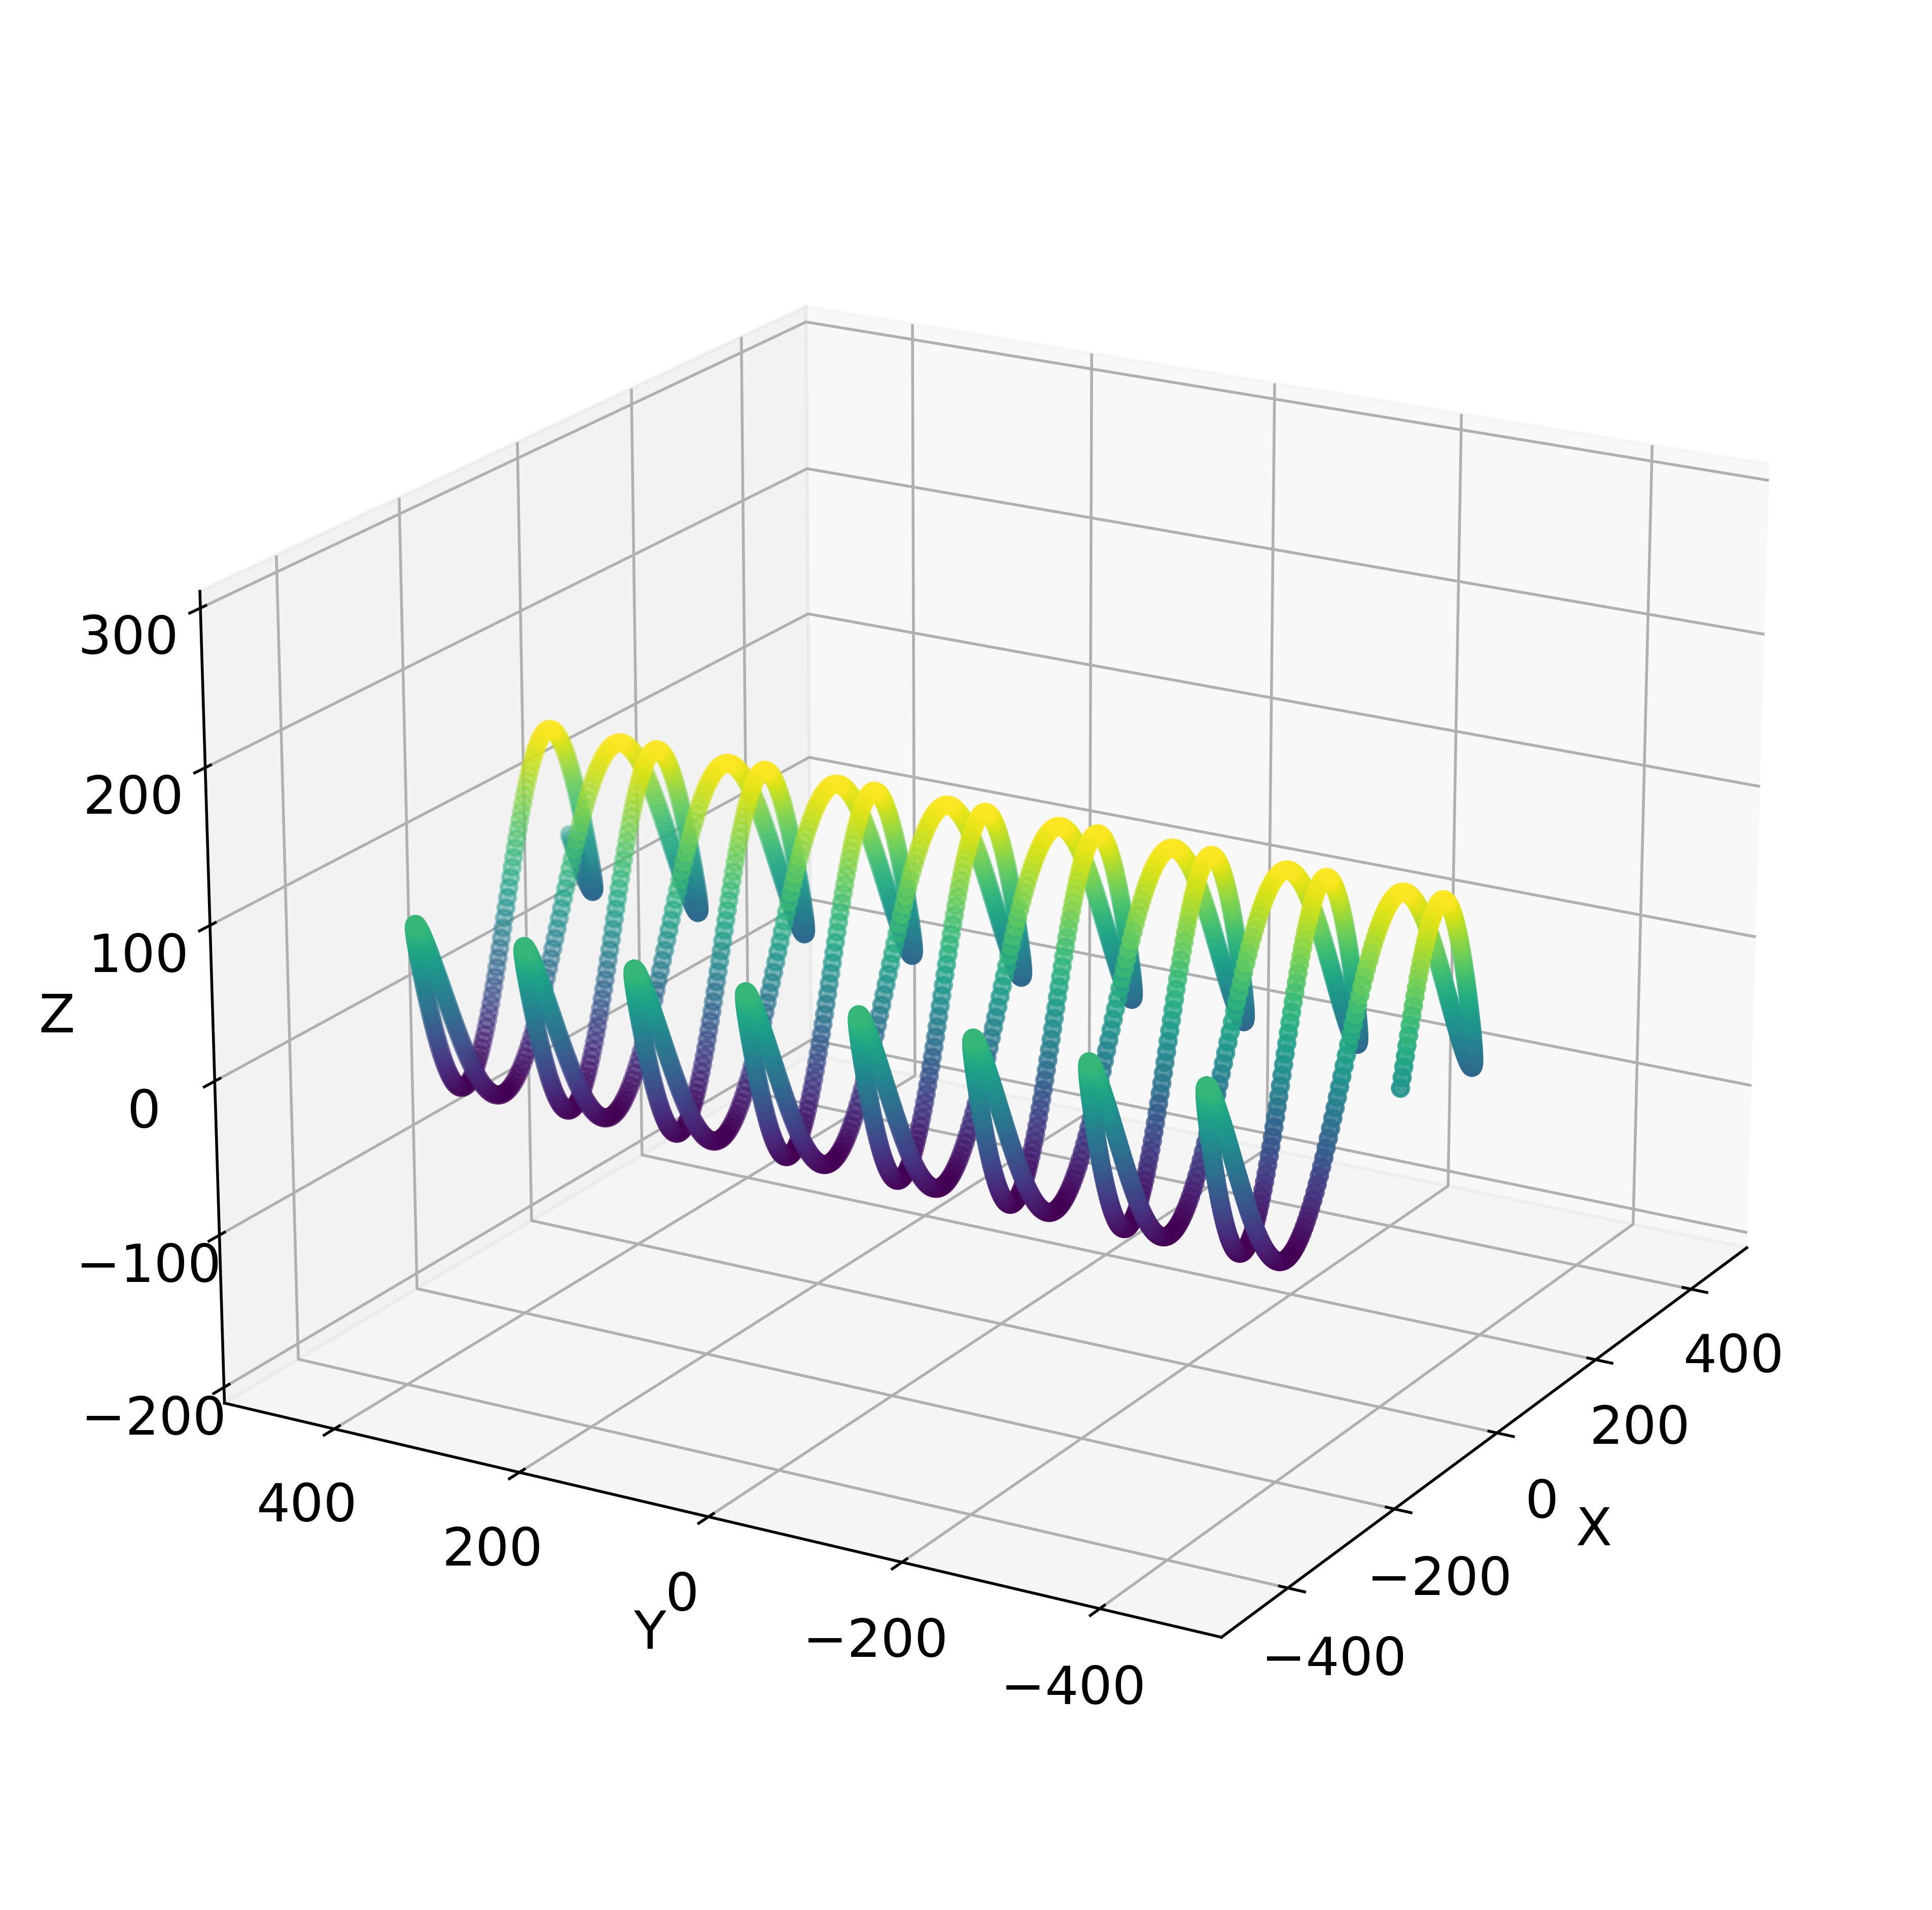
\includegraphics[width=\textwidth]{figures/path3_kipp_0.png}
		\caption{sdfgsdfg}
		\label{sdfgsdfg}
	\end{minipage}\par
	\vskip\floatsep% normal separation between figures
	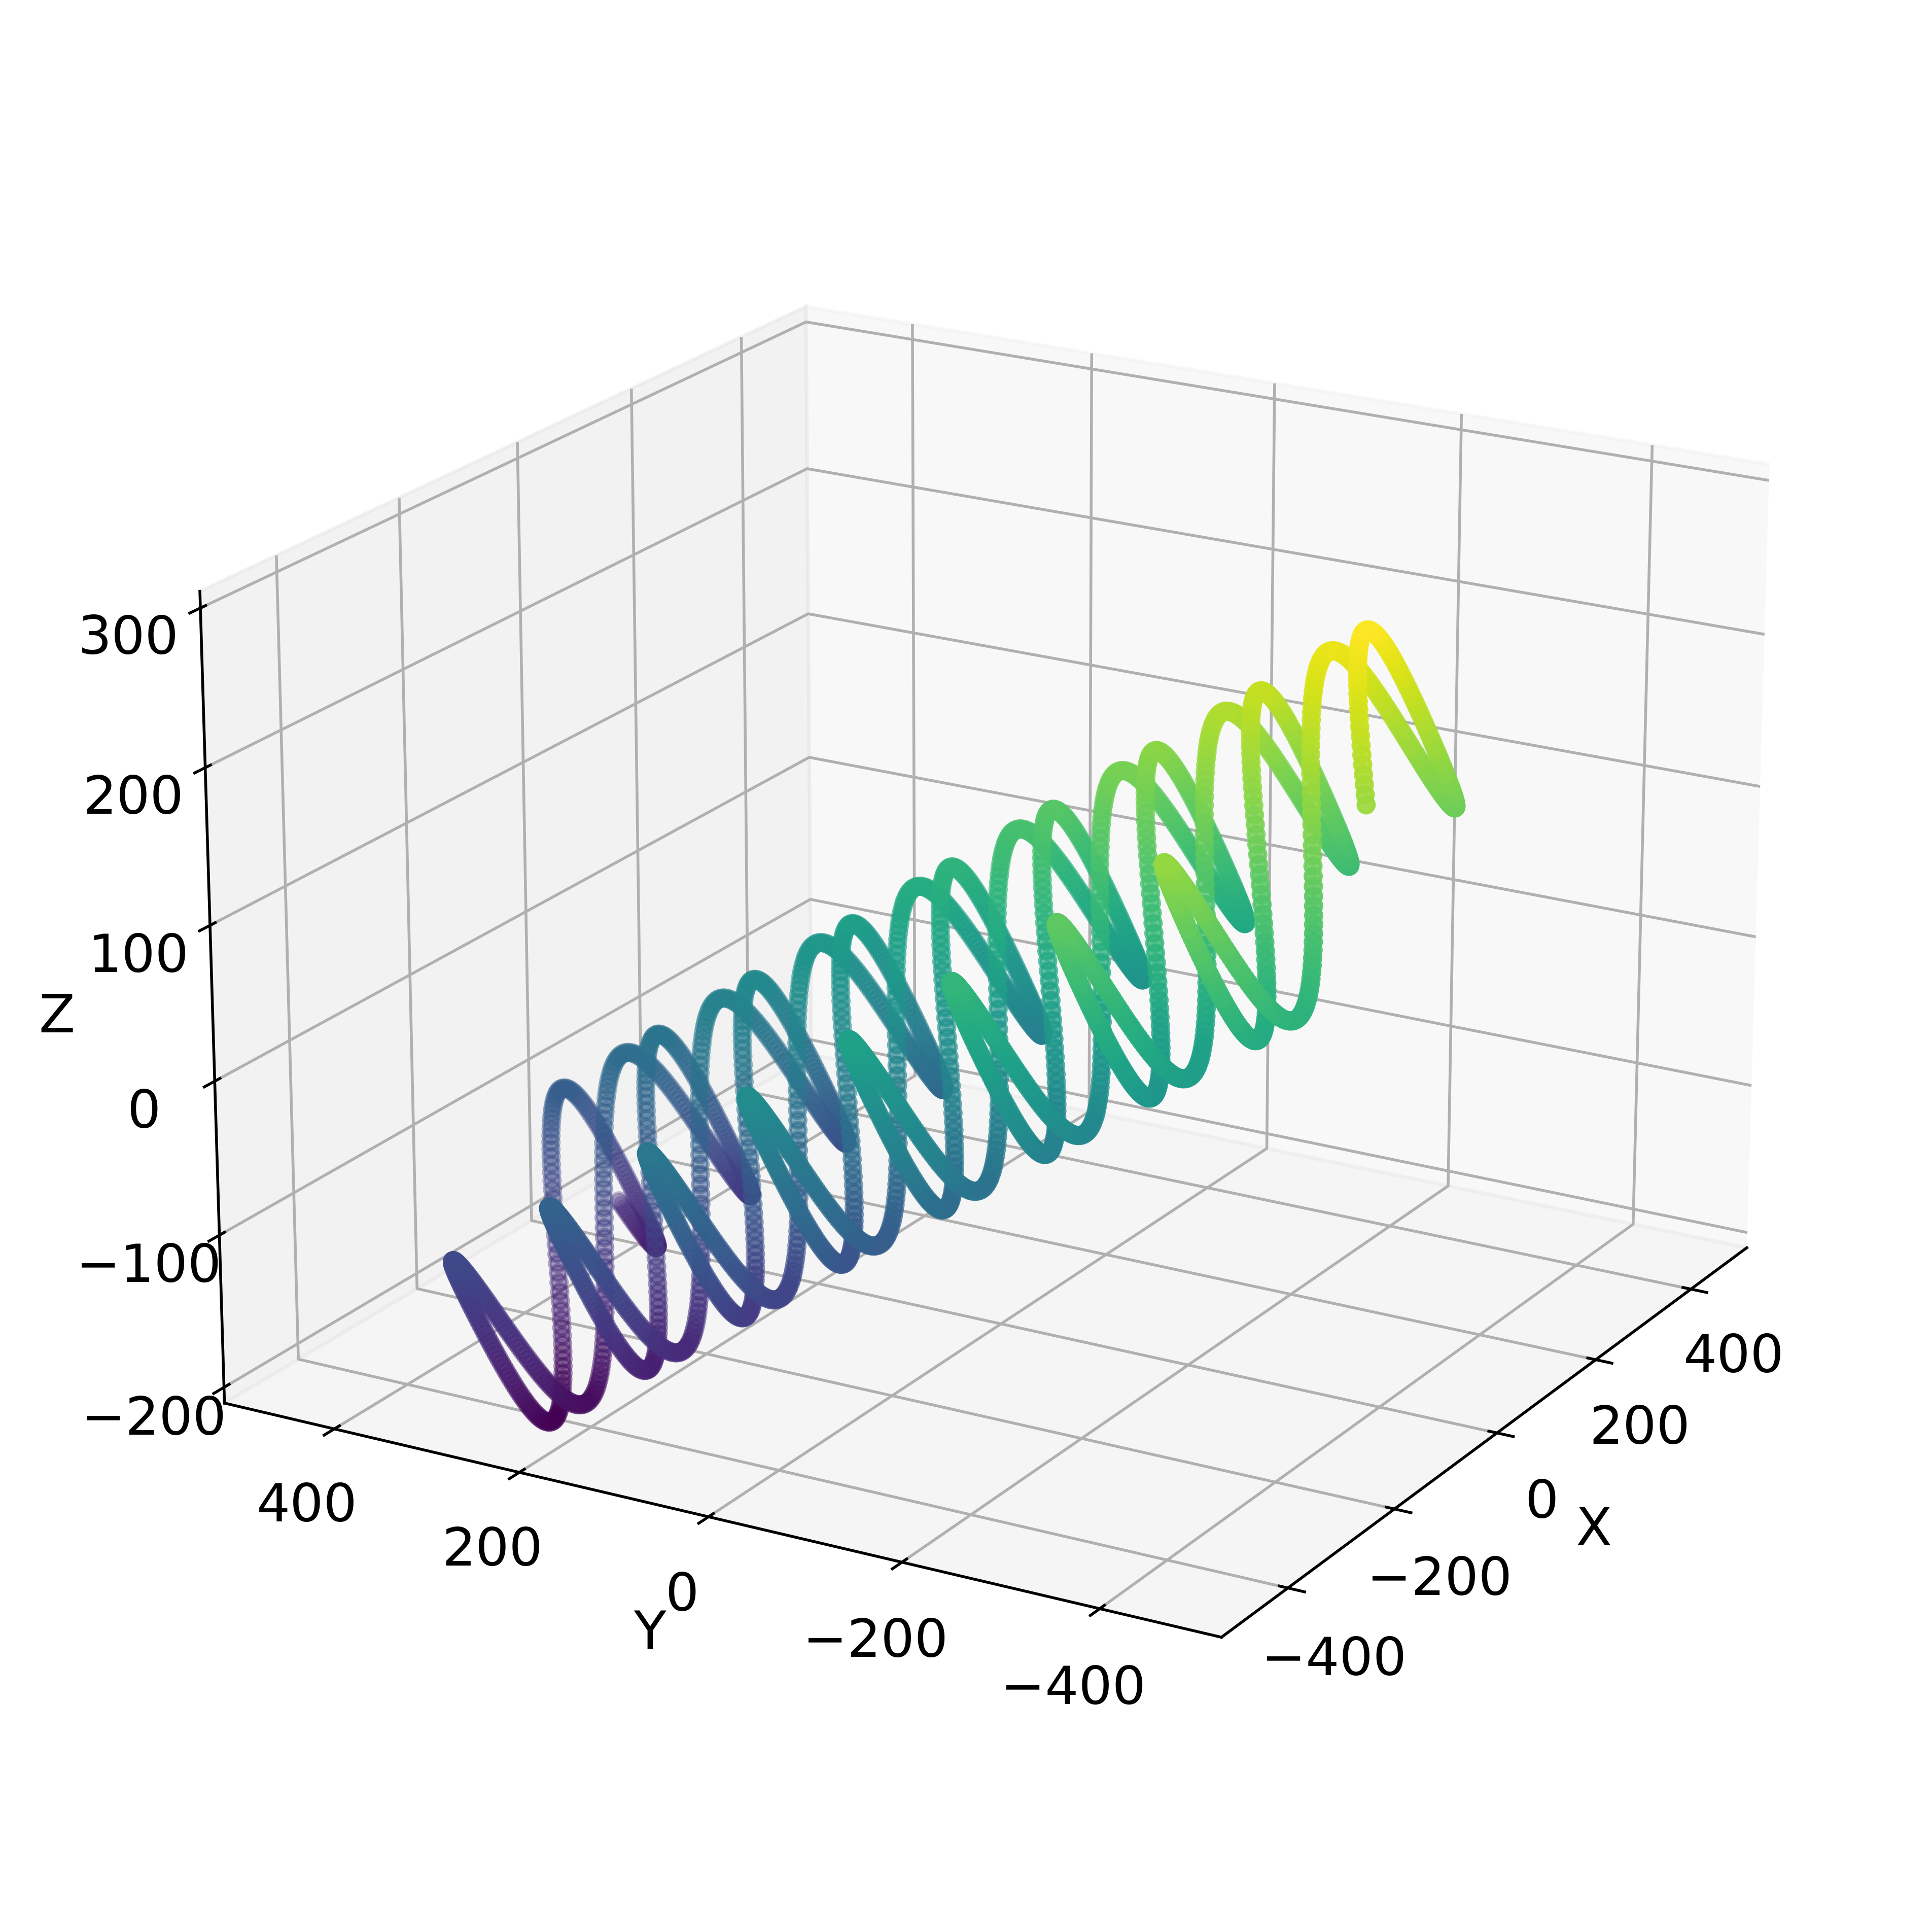
\includegraphics[width=0.5\textwidth]{figures/path3_kipp_-25.png}
	
	\caption{sdfgsdf}
	\label{sdfgds}
\end{figure}



\begin{figure}[H]
	\centerline{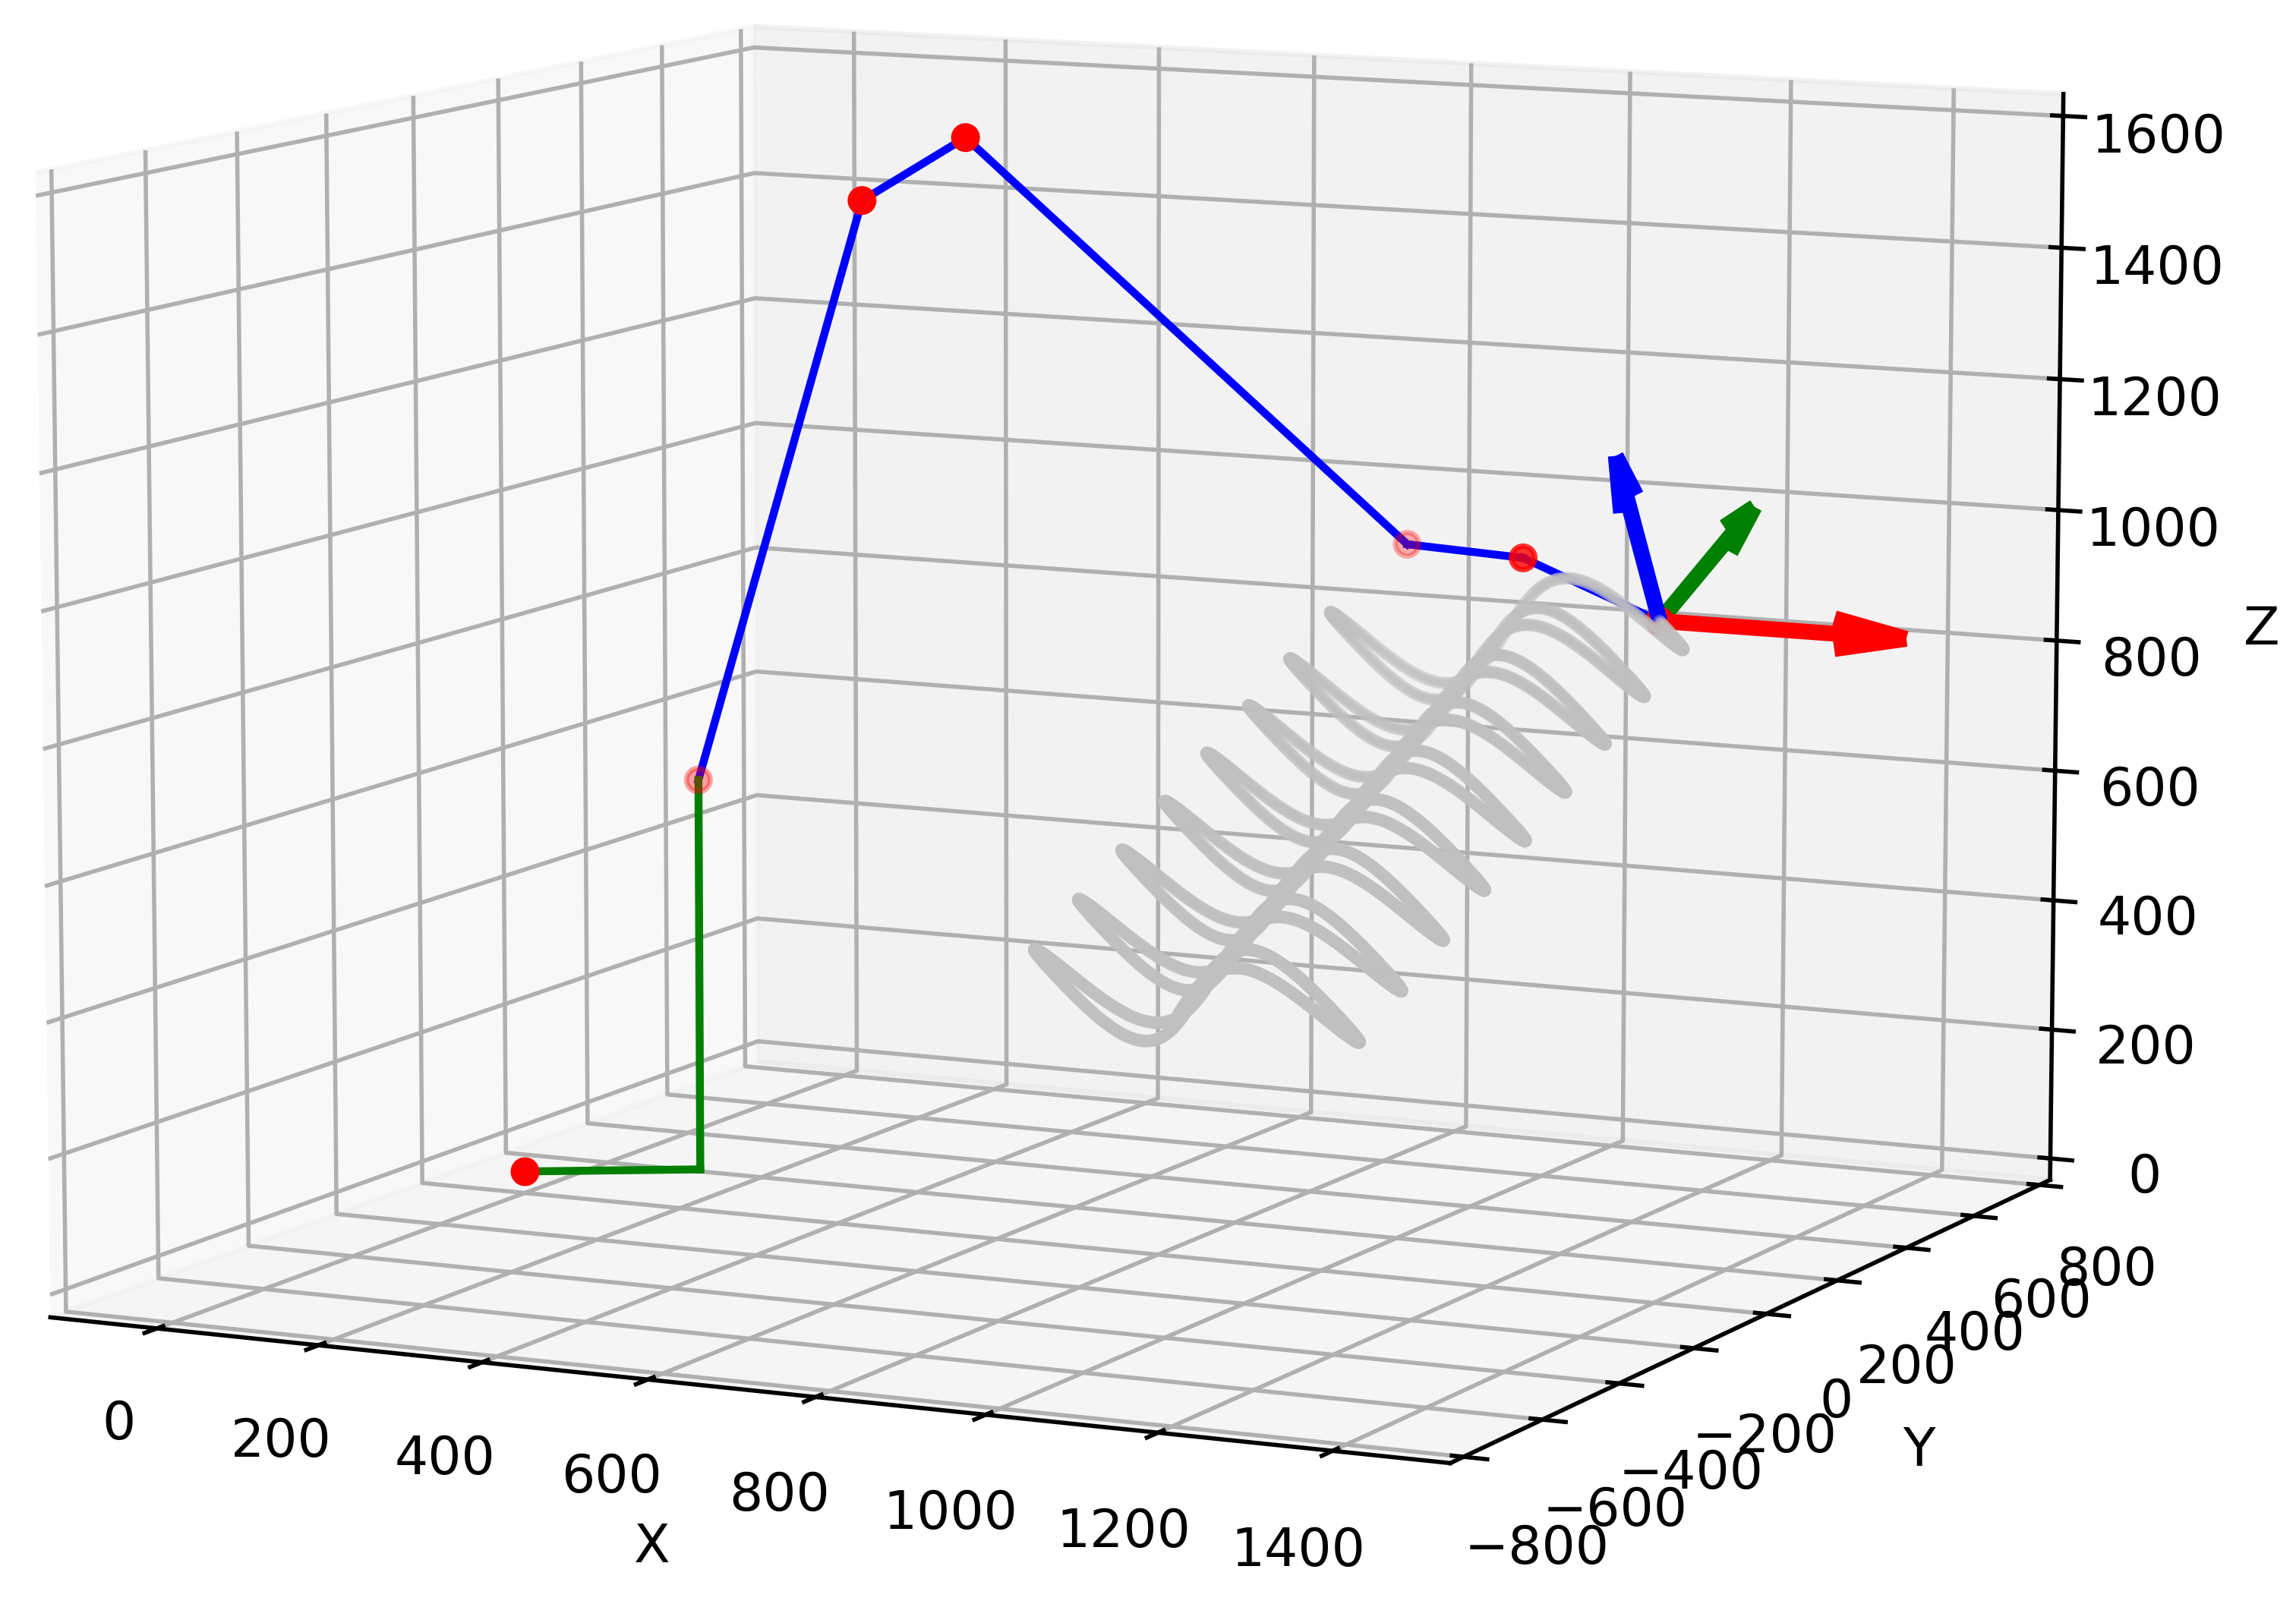
\includegraphics[width=0.9\textwidth]{figures/robotANDpath3_25.png}}
	\caption{sdfafsdfasdggsdf}
	\label{dasdfgadfgvsf}
\end{figure}


\subsection{Boundary Condition Optimization }

\section{Analysis and Discussion of the results}%


\subsection{Analysis}
\subsection{Discussion}%